\begin{center}
\begin{minipage}[b]{0.98\textwidth}
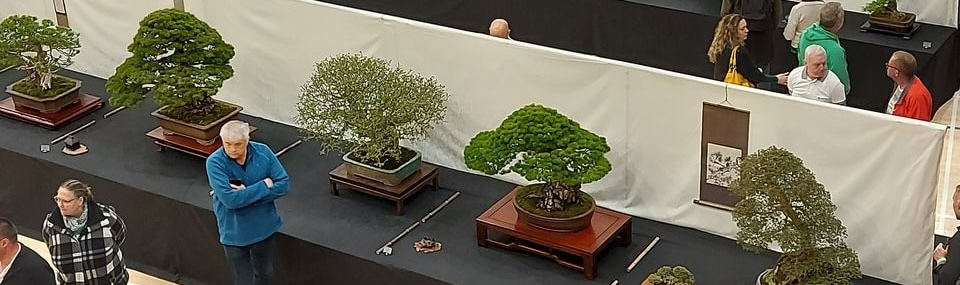
\includegraphics[angle=0,origin=c,width=1.0\textwidth]{2025_05/res/expo_k2_bonsai_expo}
\end{minipage}

\medskip
\begin{minipage}[b]{.48\textwidth}
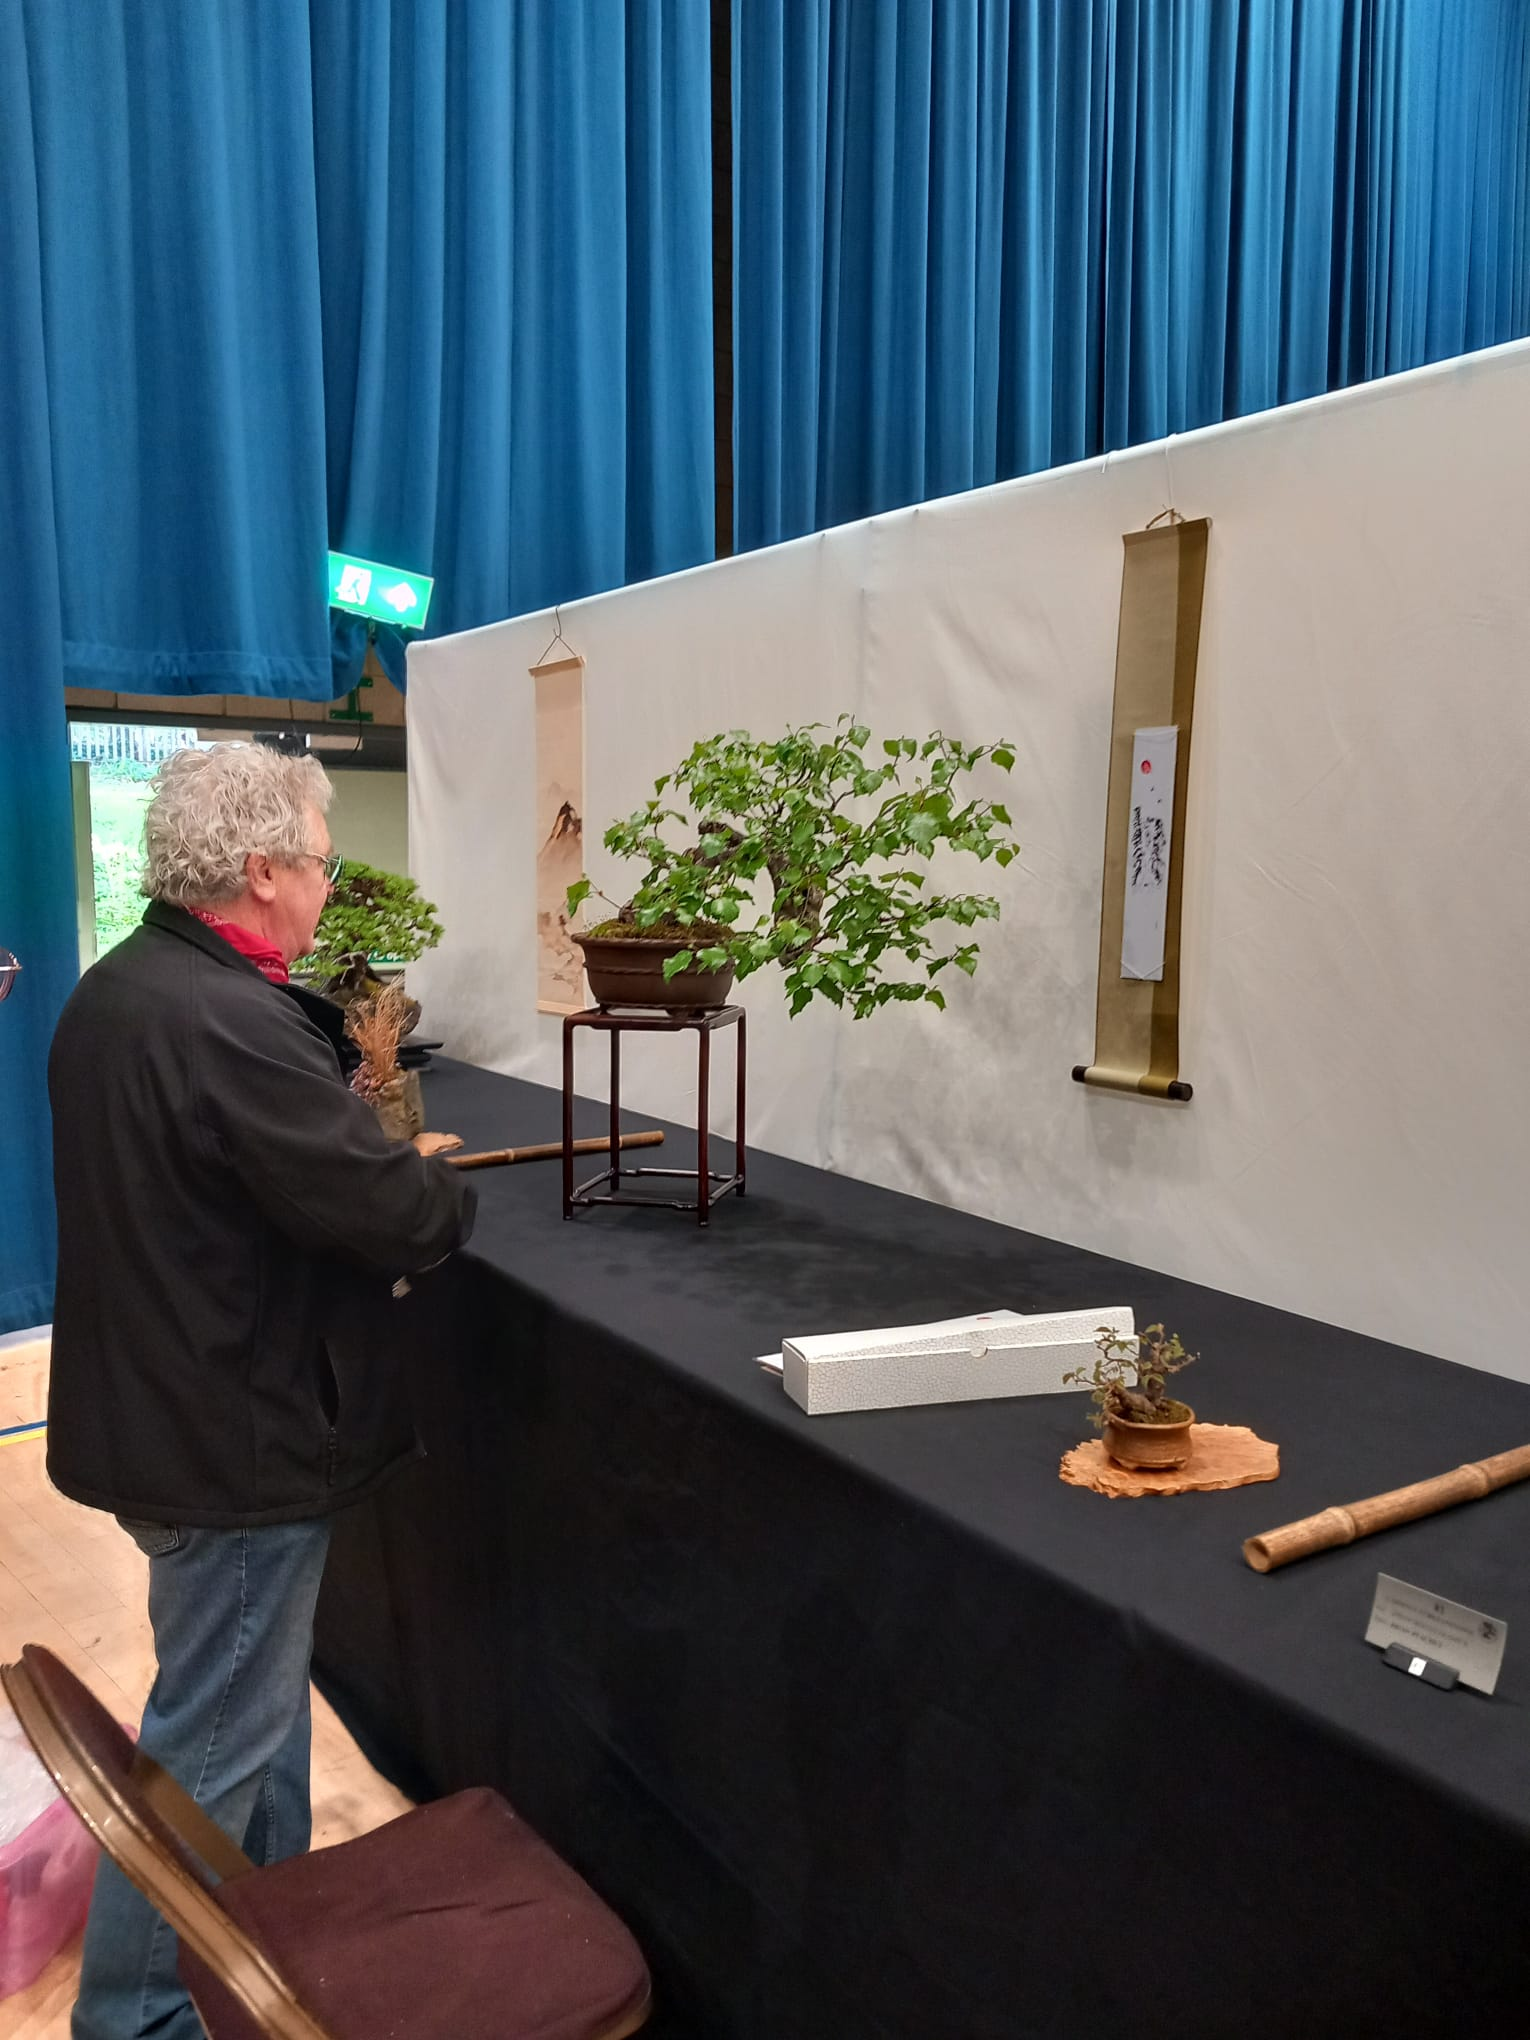
\includegraphics[angle=0,origin=c,width=1.0\textwidth]{2025_05/res/expo_prepping_tony}
\end{minipage}\quad
\begin{minipage}[b]{.48\textwidth}
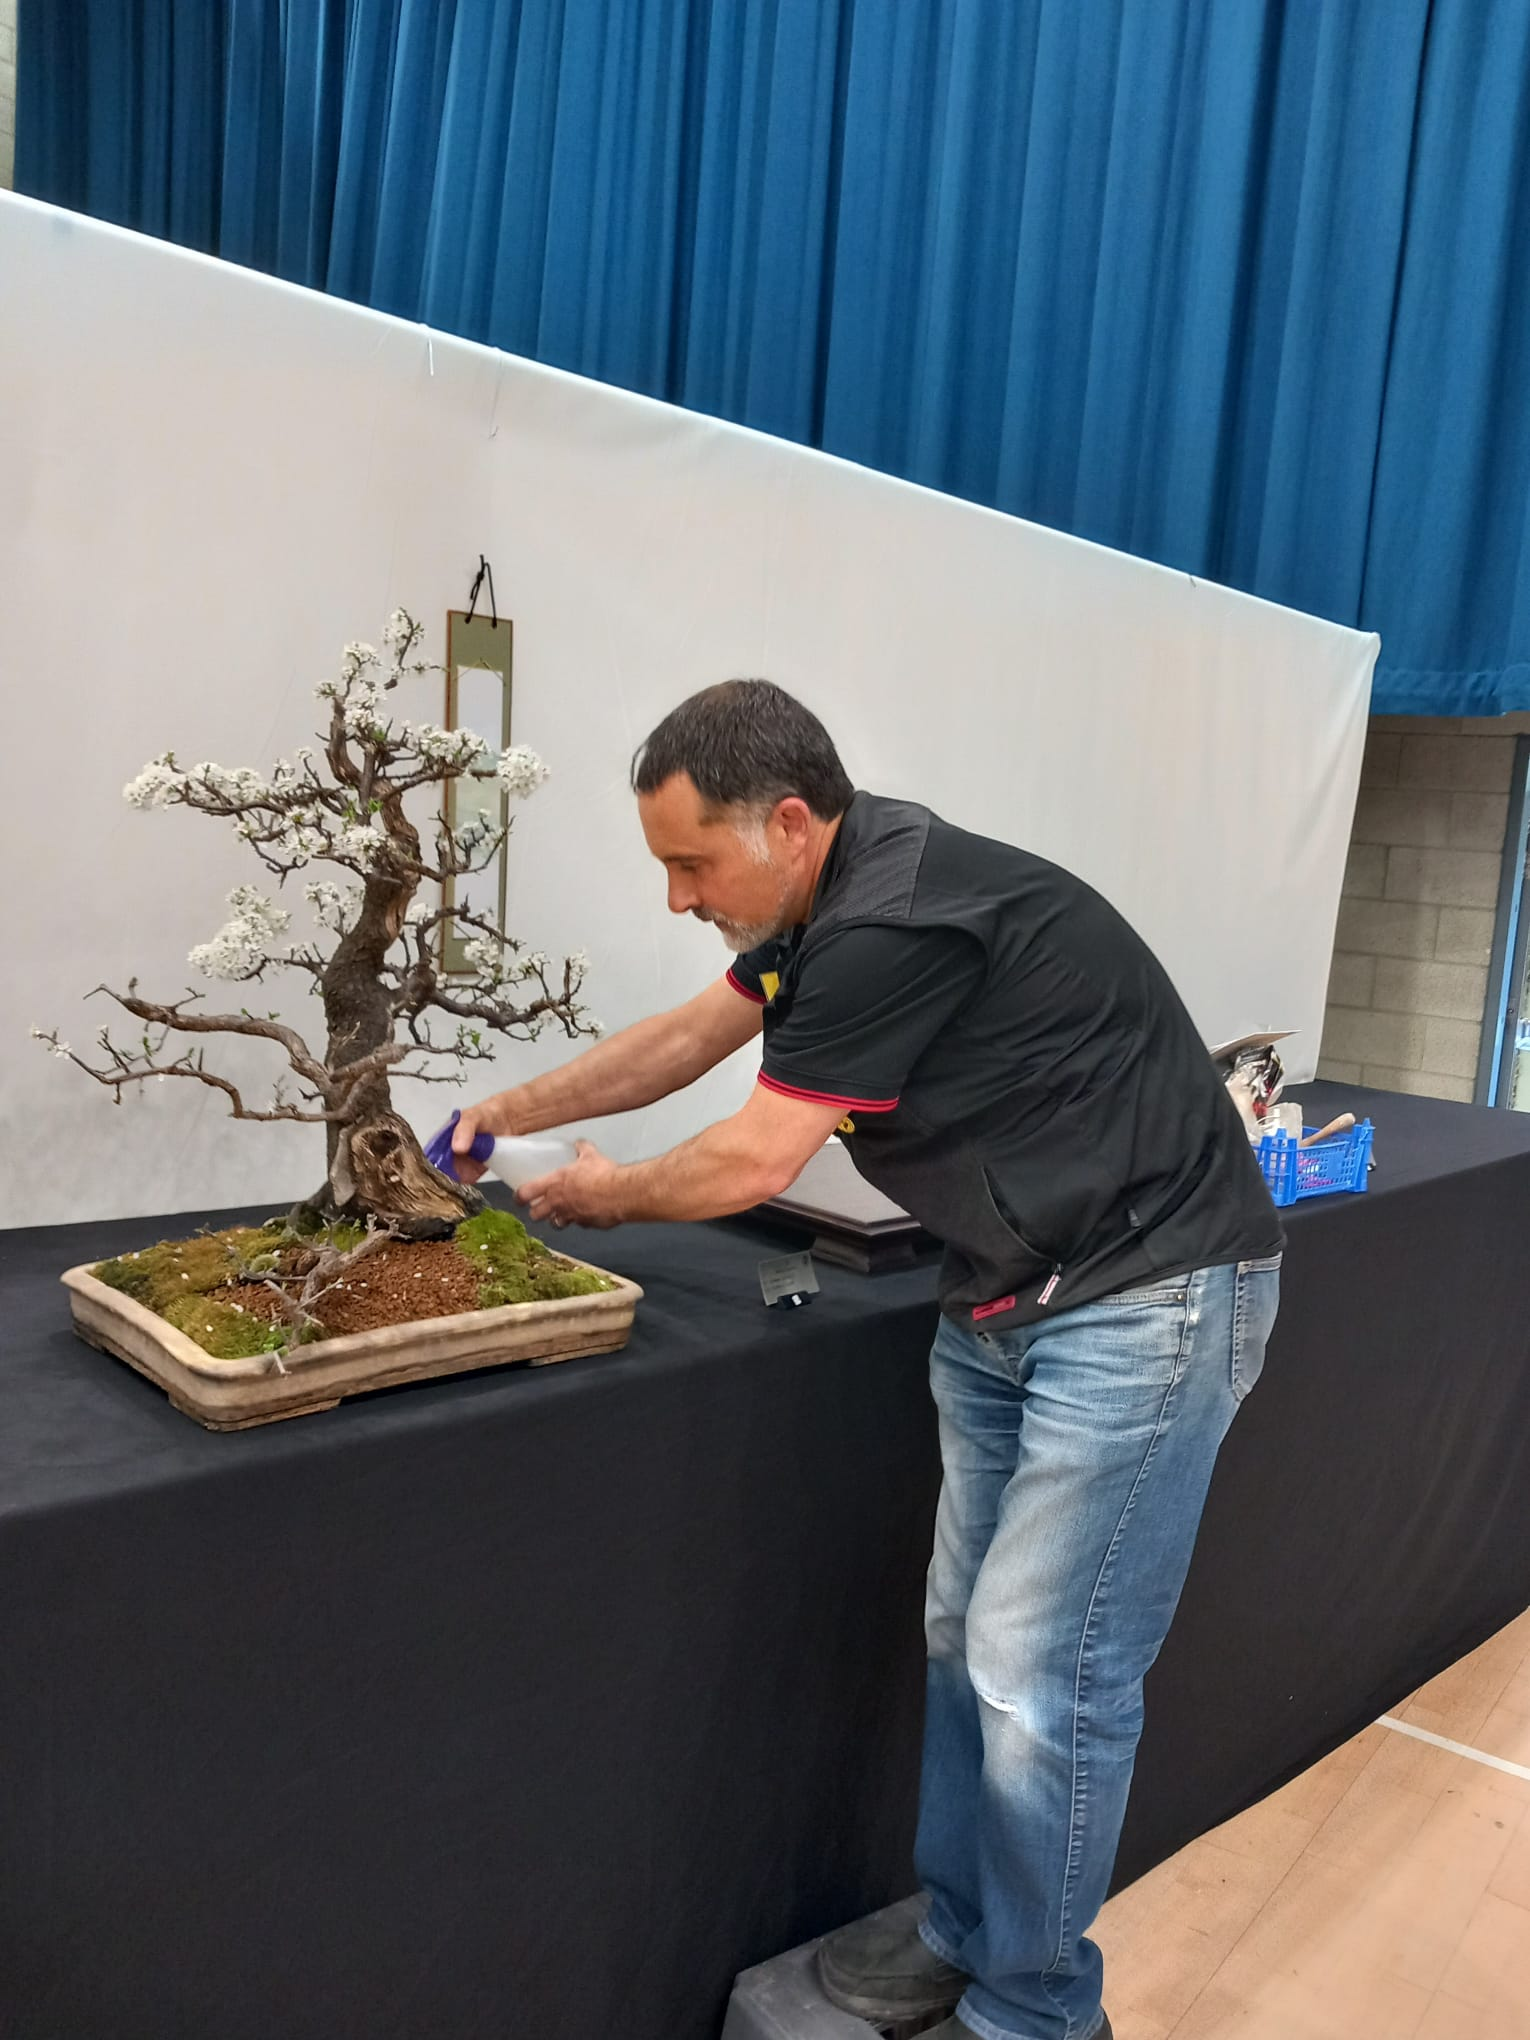
\includegraphics[angle=0,origin=c,width=1.0\textwidth]{2025_05/res/expo_prepping_nick}
\end{minipage}

\medskip
\emph{Tony and Nick, flying the Twickenham flag in Crawley as they put the final touches on their displays.}
\end{center}
\pagebreak



\topic{Tony Ulatowski --- Silver Birch \textit{(Betula pendula)}}
\vspace{-1em}
\begin{window}[%
    2,l,%
    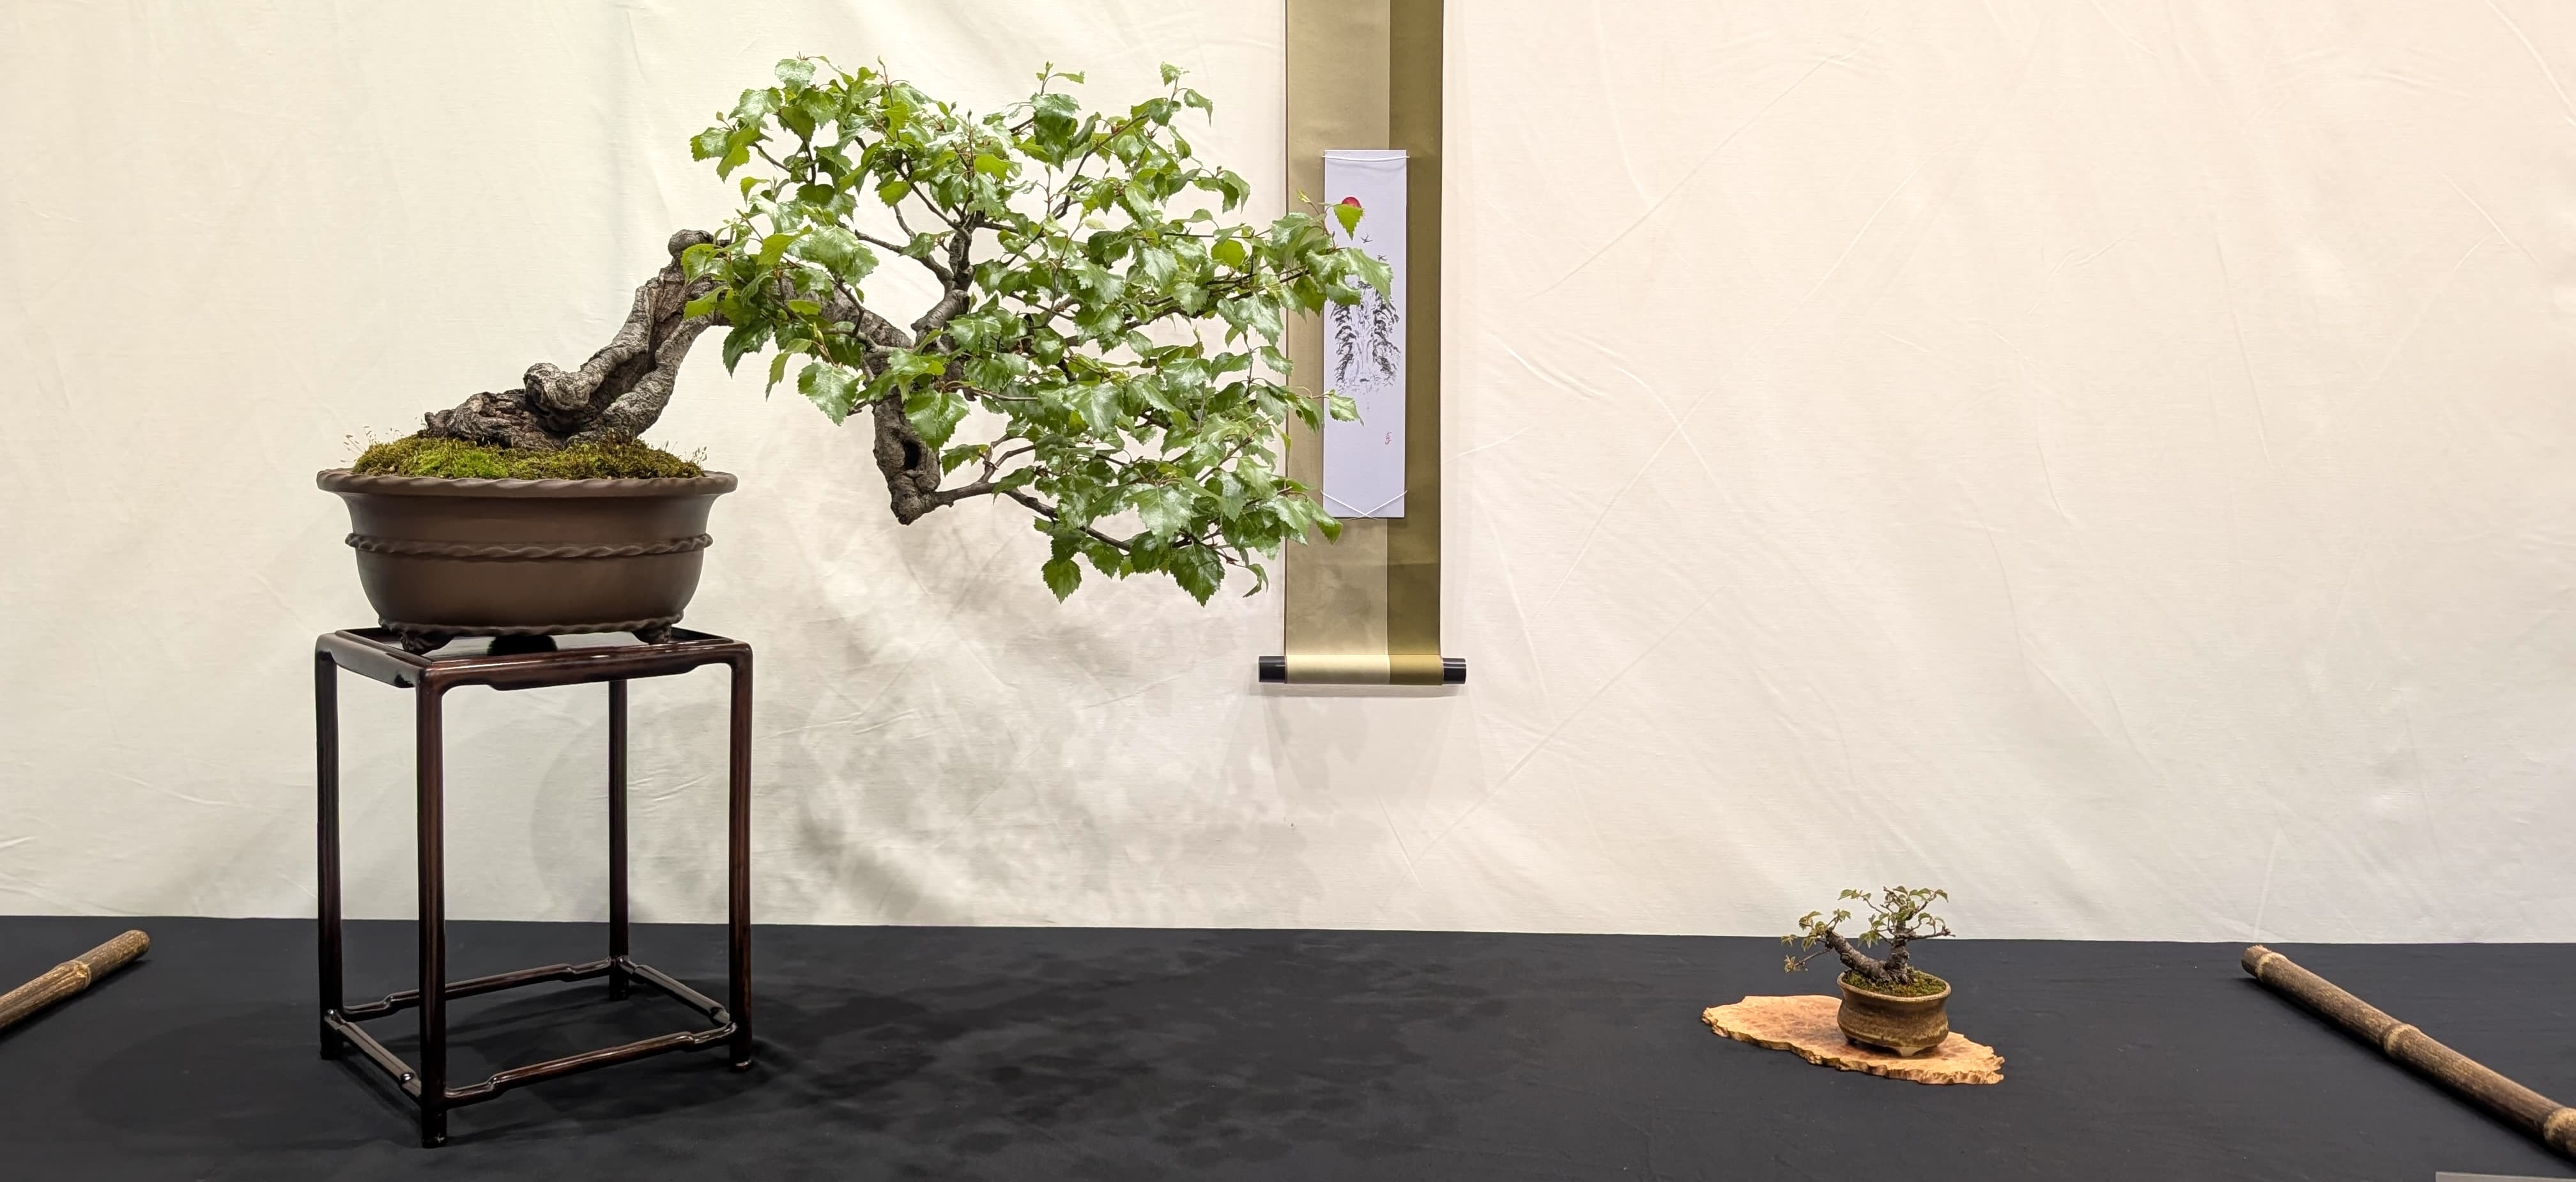
\includegraphics[width=1.0\columnwidth]{2025_05/res/expo_tony_birch},%
]
\end{window}
\noindent
Chairman of Twickenham Bonsai Club, \textbf{Tony Ulatowski}, presented two striking trees at the K2 Expo, beginning with his remarkable \textbf{Silver Birch}.
Owned for over a decade, this tree is particularly eye\--catching due to its \textbf{almost entirely hollow trunk}, a feature that adds dramatic texture and aged character.
Originally styled in a cascading form, the tree lost its bottom branch---a common fate with birches---and Tony considered parting with it.
But then, in true bonsai spirit, he rediscovered its potential.
After significant restyling and a complete reimagining of its structure, the tree re\--emerged more elegant than ever.
Now potted in a \textbf{refined, high\--quality Japanese container}, it stood proudly at K2---a testament to resilience and vision.
\textit{``I fell out of love with it\dots then back in love with it,''} Tony laughs, \textit{``but don't tell my wife!''}

\medskip
\topic{Japanese Maple \textit{(Acer palmatum)}}
\vspace{-1em}
\begin{window}[%
    2,l,%
    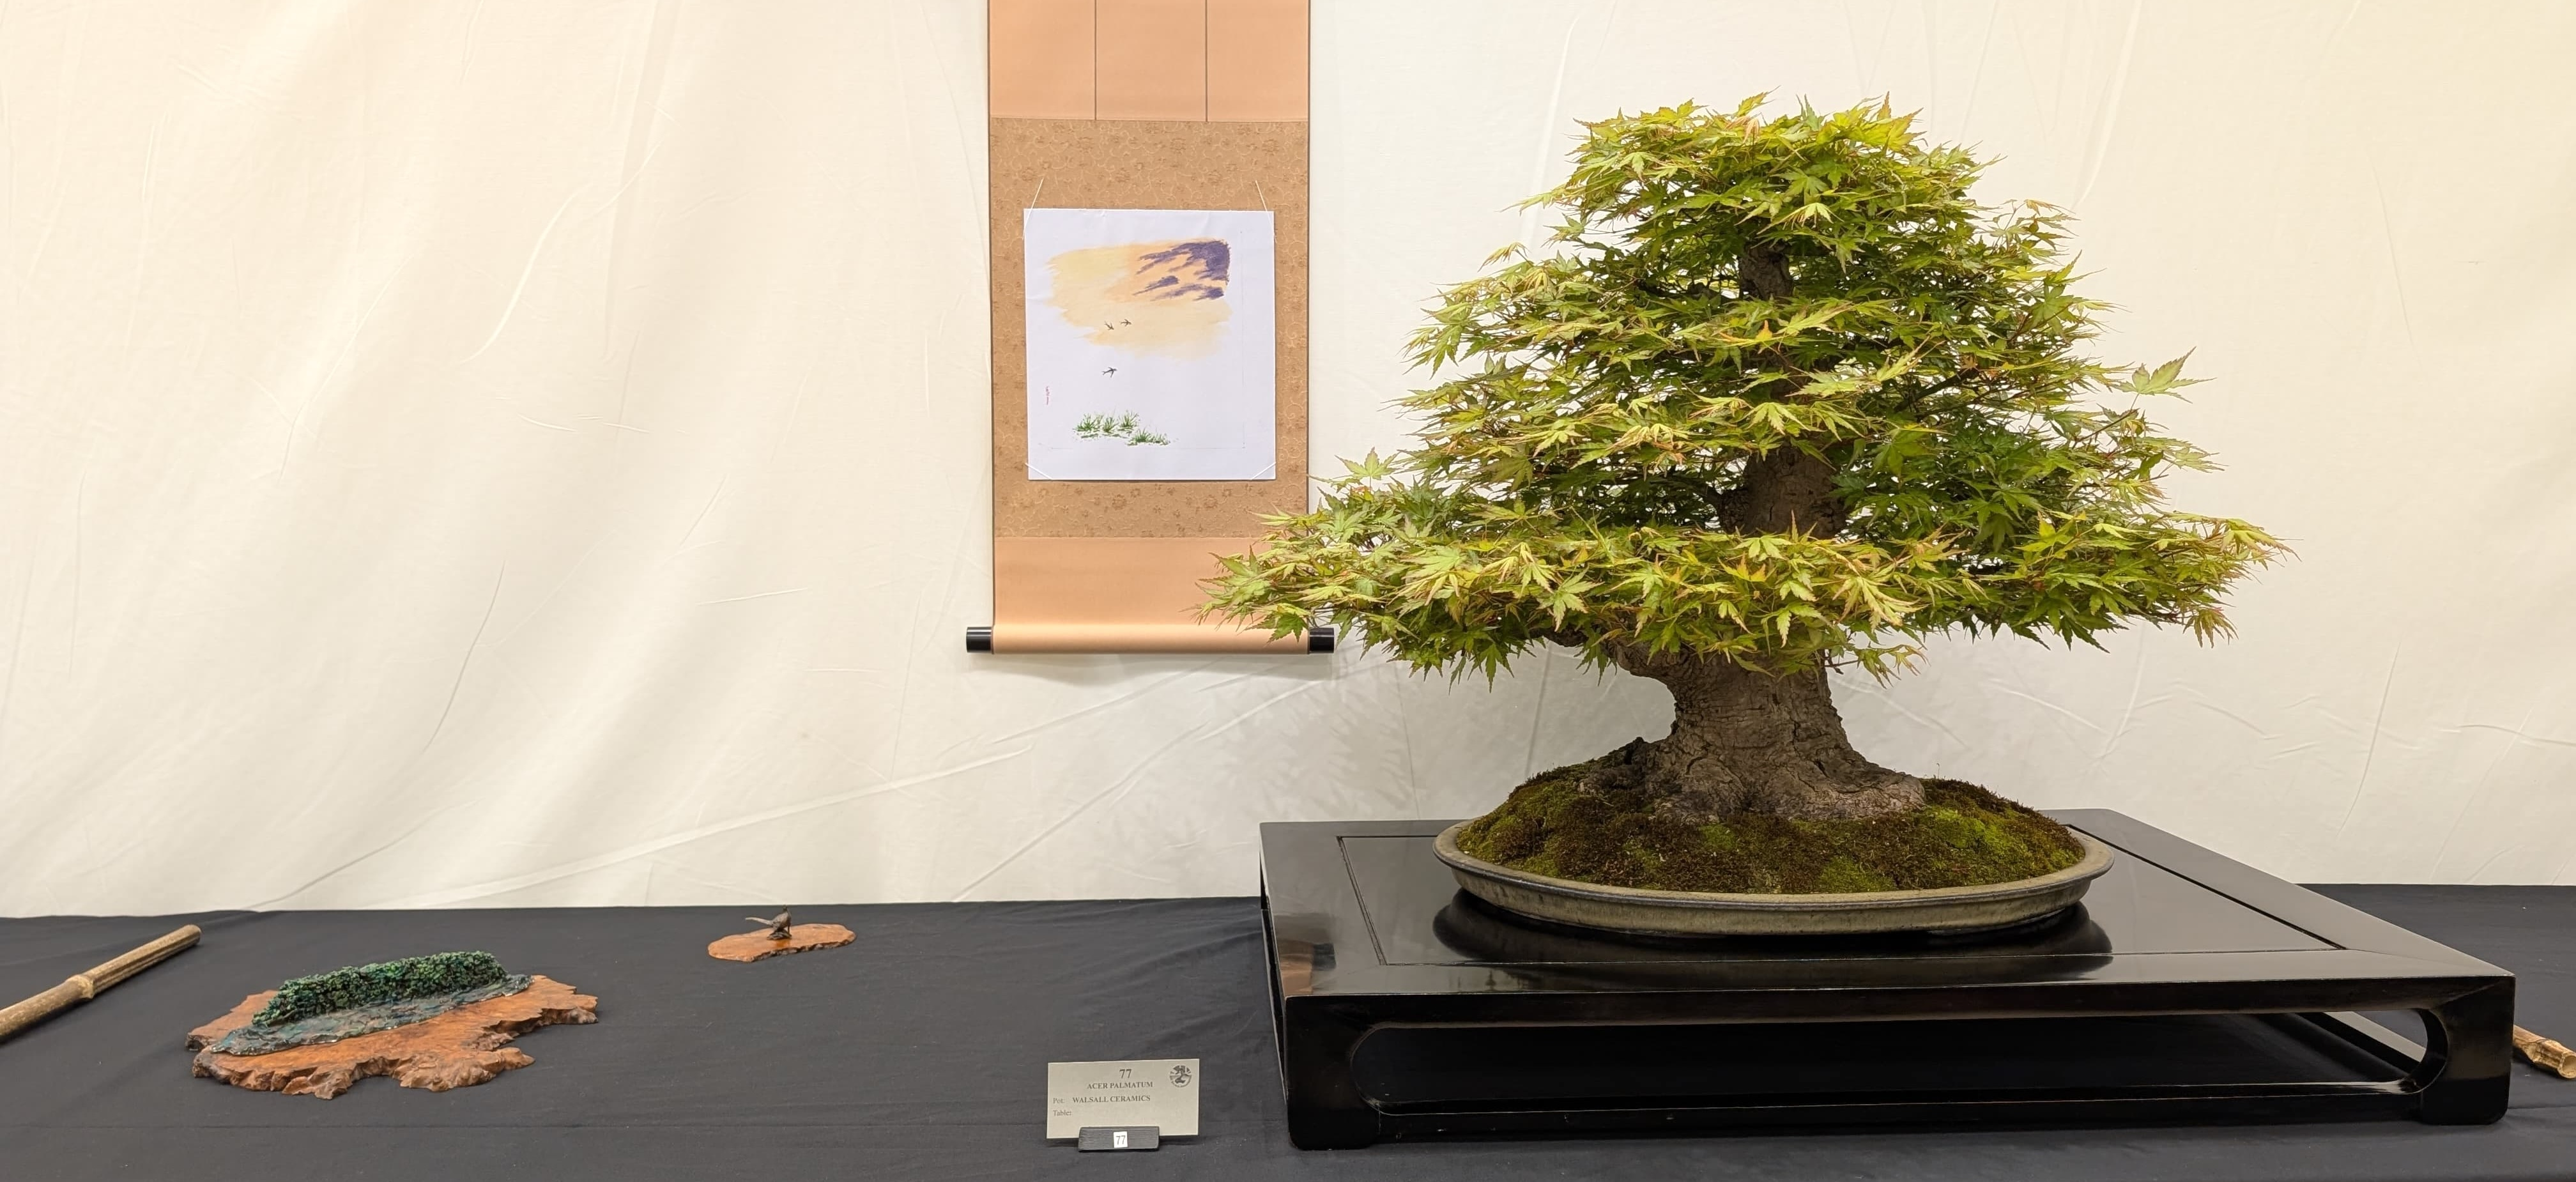
\includegraphics[width=1.0\columnwidth]{2025_05/res/expo_tony_maple},%
]
\end{window}
\noindent
Tony's second tree, a powerful \textbf{Japanese Maple}, has been in his care for around five years.
For much of that time it was focused on gaining strength in a training pot.
Only this year was it repotted into its current \textbf{elegant shallow container}, a step that marked a significant milestone in its development.
The tree has recently seen noticeable improvement in \textbf{branch ramification}, and Tony is excited about the ongoing work. \textit{``It's a cracker,''} he says with characteristic humour---a phrase that couldn't be more fitting for such a refined and balanced composition.
\pagebreak



\topic{Nick Lloyd, Secretary --- Blackthorn \textit{(Prunus spinosa)}}
\vspace{-1em}
\begin{window}[%
    2,l,%
    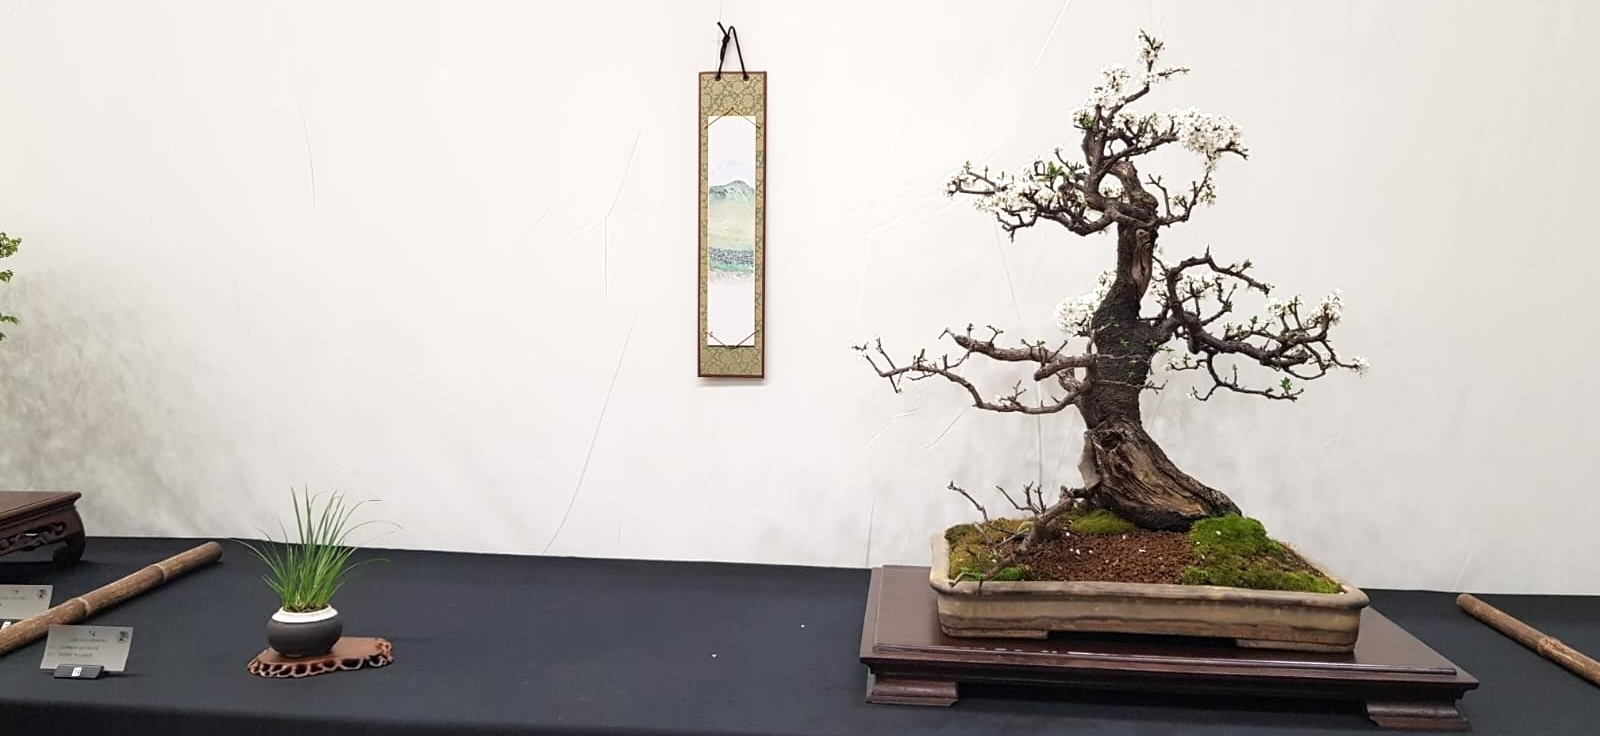
\includegraphics[width=1.0\columnwidth]{2025_05/res/expo_nick_blackthorn},%
]
\end{window}
\noindent
Club Secretary \textbf{Nick Lloyd} presented a \textbf{blackthorn} (\textit{Prunus spinosa}) with a quietly dramatic presence.
Acquired around five years ago as raw material collected by Will Baddeley, the tree had never flowered and came with a weak root system --- common with blackthorns.
Since then, Nick has rebuilt its foundation, encouraging strong roots and training suckers as future bonsai.
A past stump near the base and the apex have both been carefully carved under Will's suggestion, adding age and texture.
Now a regular flowerer, the tree still has plans ahead: Nick aims to refine the branch structure and adjust the planting angle slightly, having lost a large root in a recent repot.
This tree is a patient work in progress --- and clearly one he enjoys returning to.

\medskip
\topic{Liz Panton --- Korean Hornbeam \textit{(Carpinus turczaninowii)}}
\vspace{-1em}
\begin{window}[%
    2,l,%
    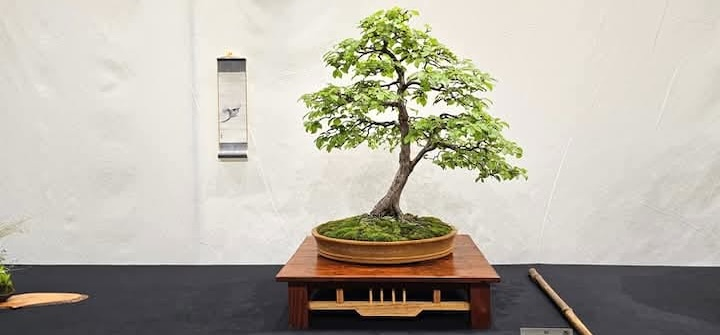
\includegraphics[width=1.0\columnwidth]{2025_05/res/expo_liz_hornbeam},%
]
\end{window}
\noindent
Online member and Chairman of the Chichester Club, \textbf{Liz Panton} is no stranger to the Twickenham Club nor to the show table.
Her display featured a beautifully feminine \textbf{Korean Hornbeam} (\textit{Carpinus turczaninowii}), around 40 years old and in her care for 30 of them.
It was gifted to her as raw material in thanks for helping at a bonsai event years ago, and has never once been wired --- shaped solely through thoughtful pruning.
The tree sat elegantly on a handmade stand crafted by a fellow Chichester member's husband, paired with a stunning scroll of a \textbf{long\--tailed tit in flight}, painted by our own \textbf{Nick Lloyd} --- a touch Liz said brought her real delight.
While we weren't able to capture the full display including the accent plant (apologies, Liz!), the tree's quiet maturity still shines.
Liz plans to thicken the canopy in coming years — and hopefully display it again soon.
\pagebreak



\begin{center}
\begin{minipage}[b]{.29\textwidth}
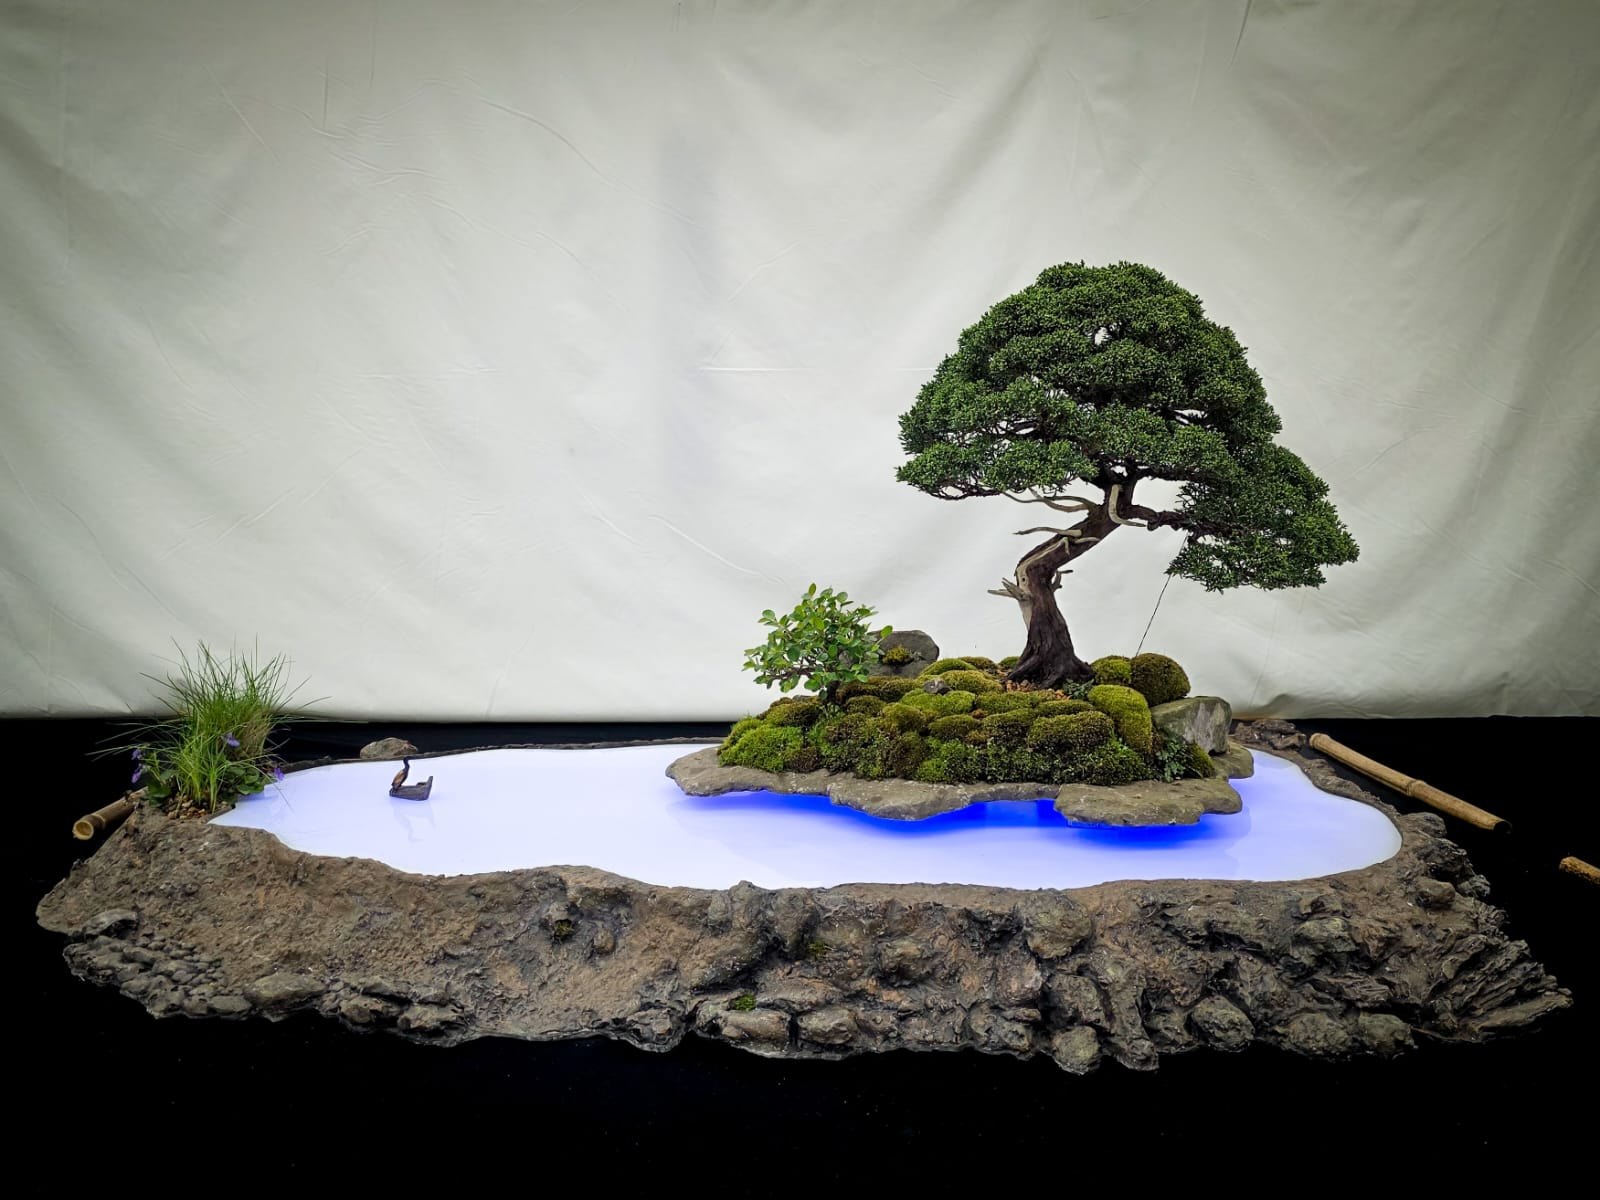
\includegraphics[angle=0,origin=c,width=1.0\textwidth]{2025_05/res/expo_11}
\end{minipage}\quad
\begin{minipage}[b]{.29\textwidth}
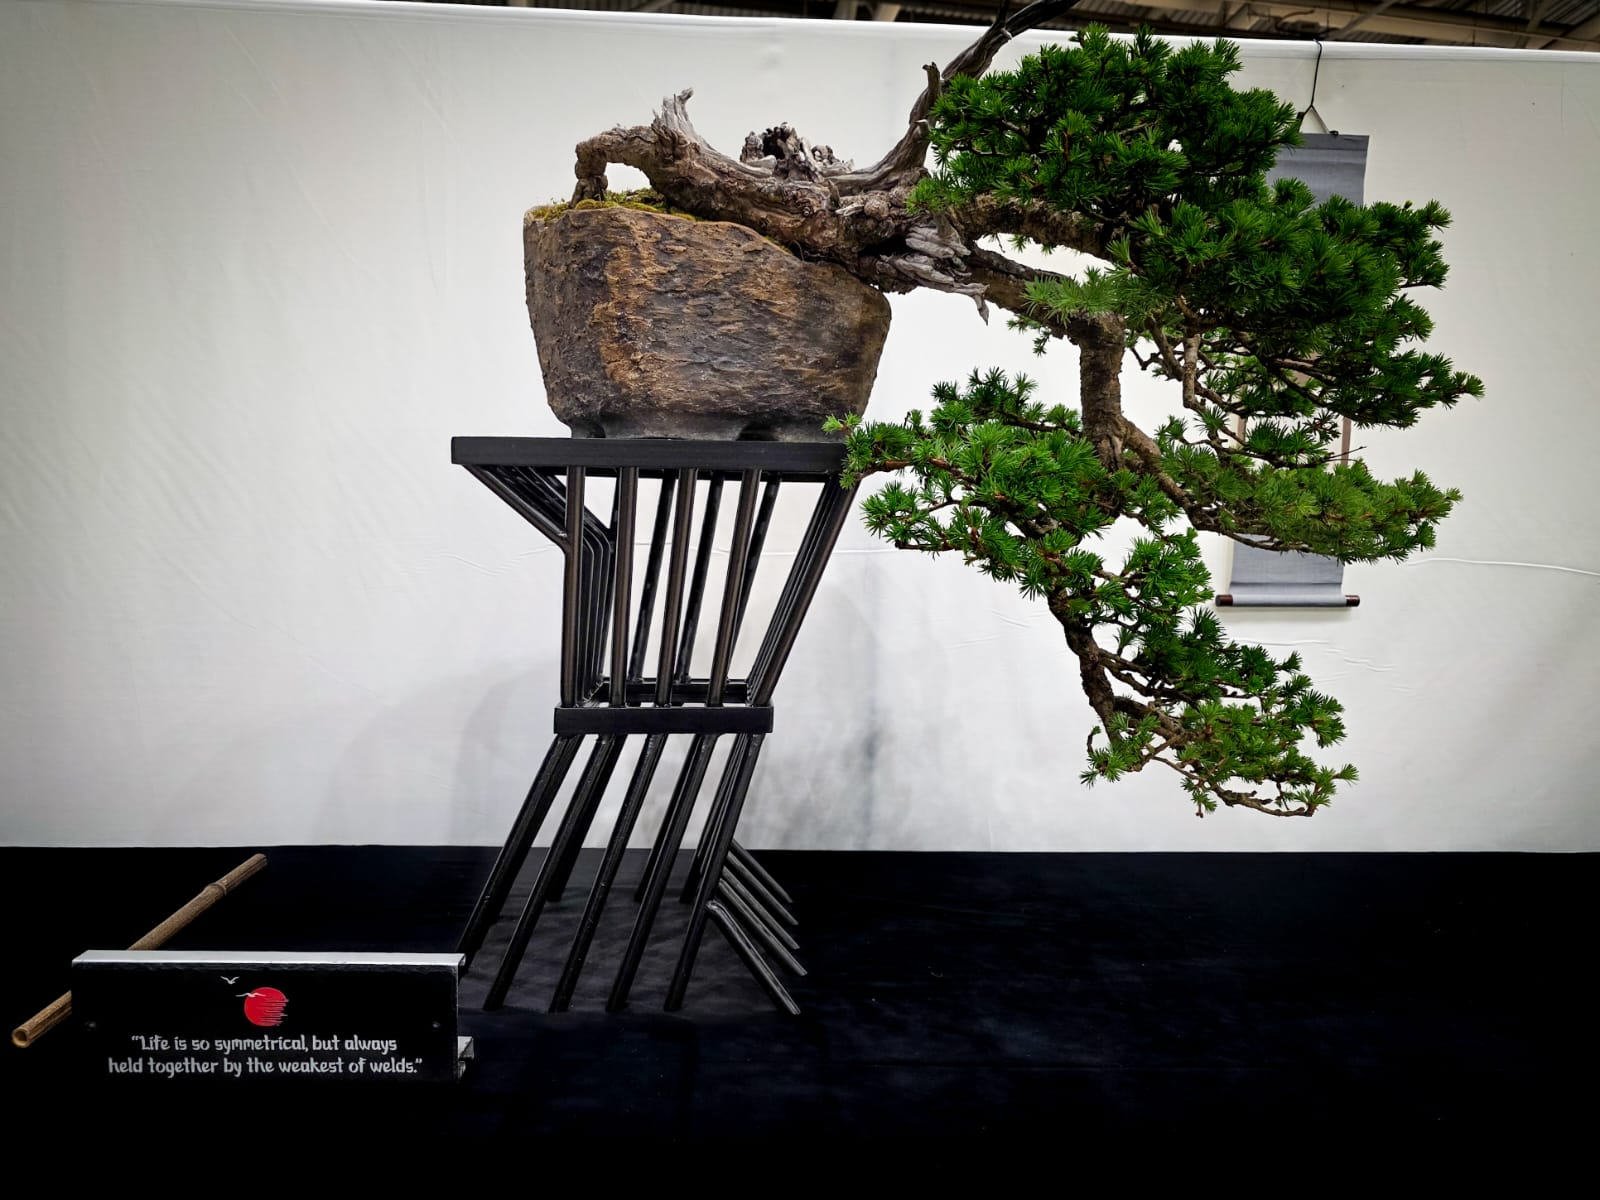
\includegraphics[angle=0,origin=c,width=1.0\textwidth]{2025_05/res/expo_02}
\end{minipage}\quad
\begin{minipage}[b]{.29\textwidth}
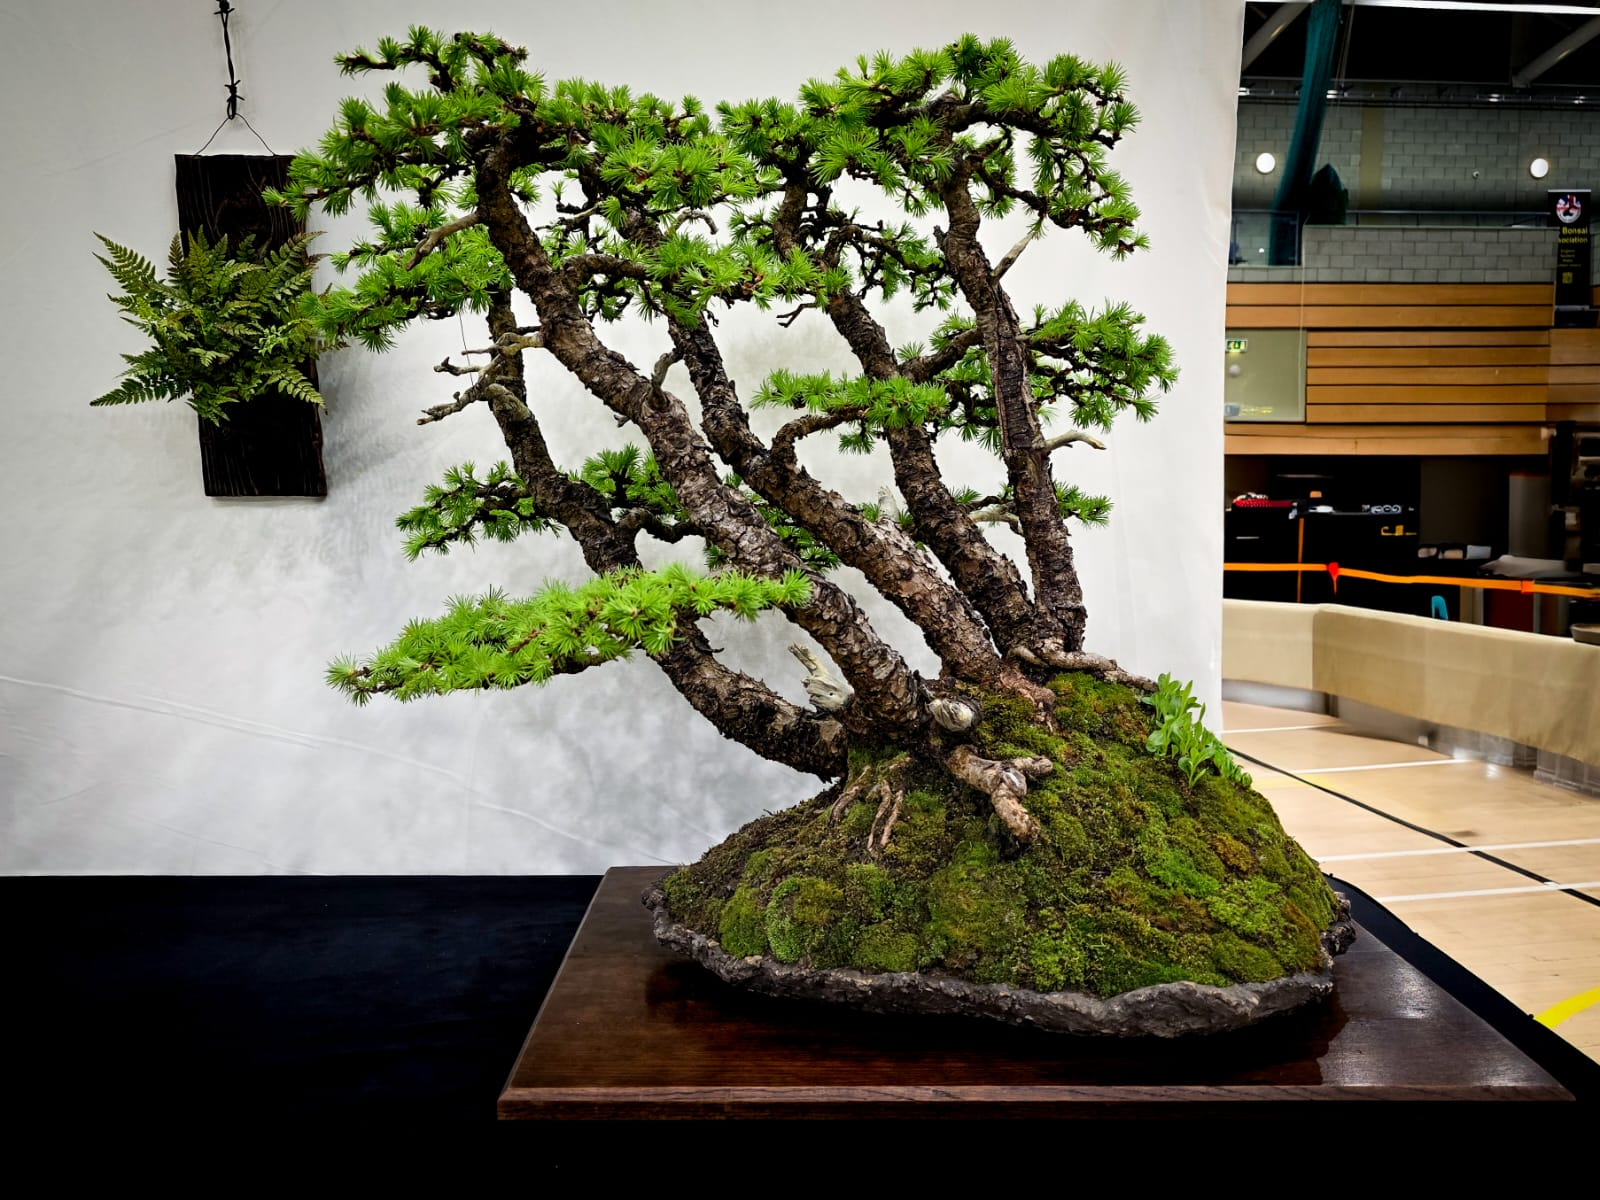
\includegraphics[angle=0,origin=c,width=1.0\textwidth]{2025_05/res/expo_05}
\end{minipage}

\medskip
\begin{minipage}[b]{.29\textwidth}
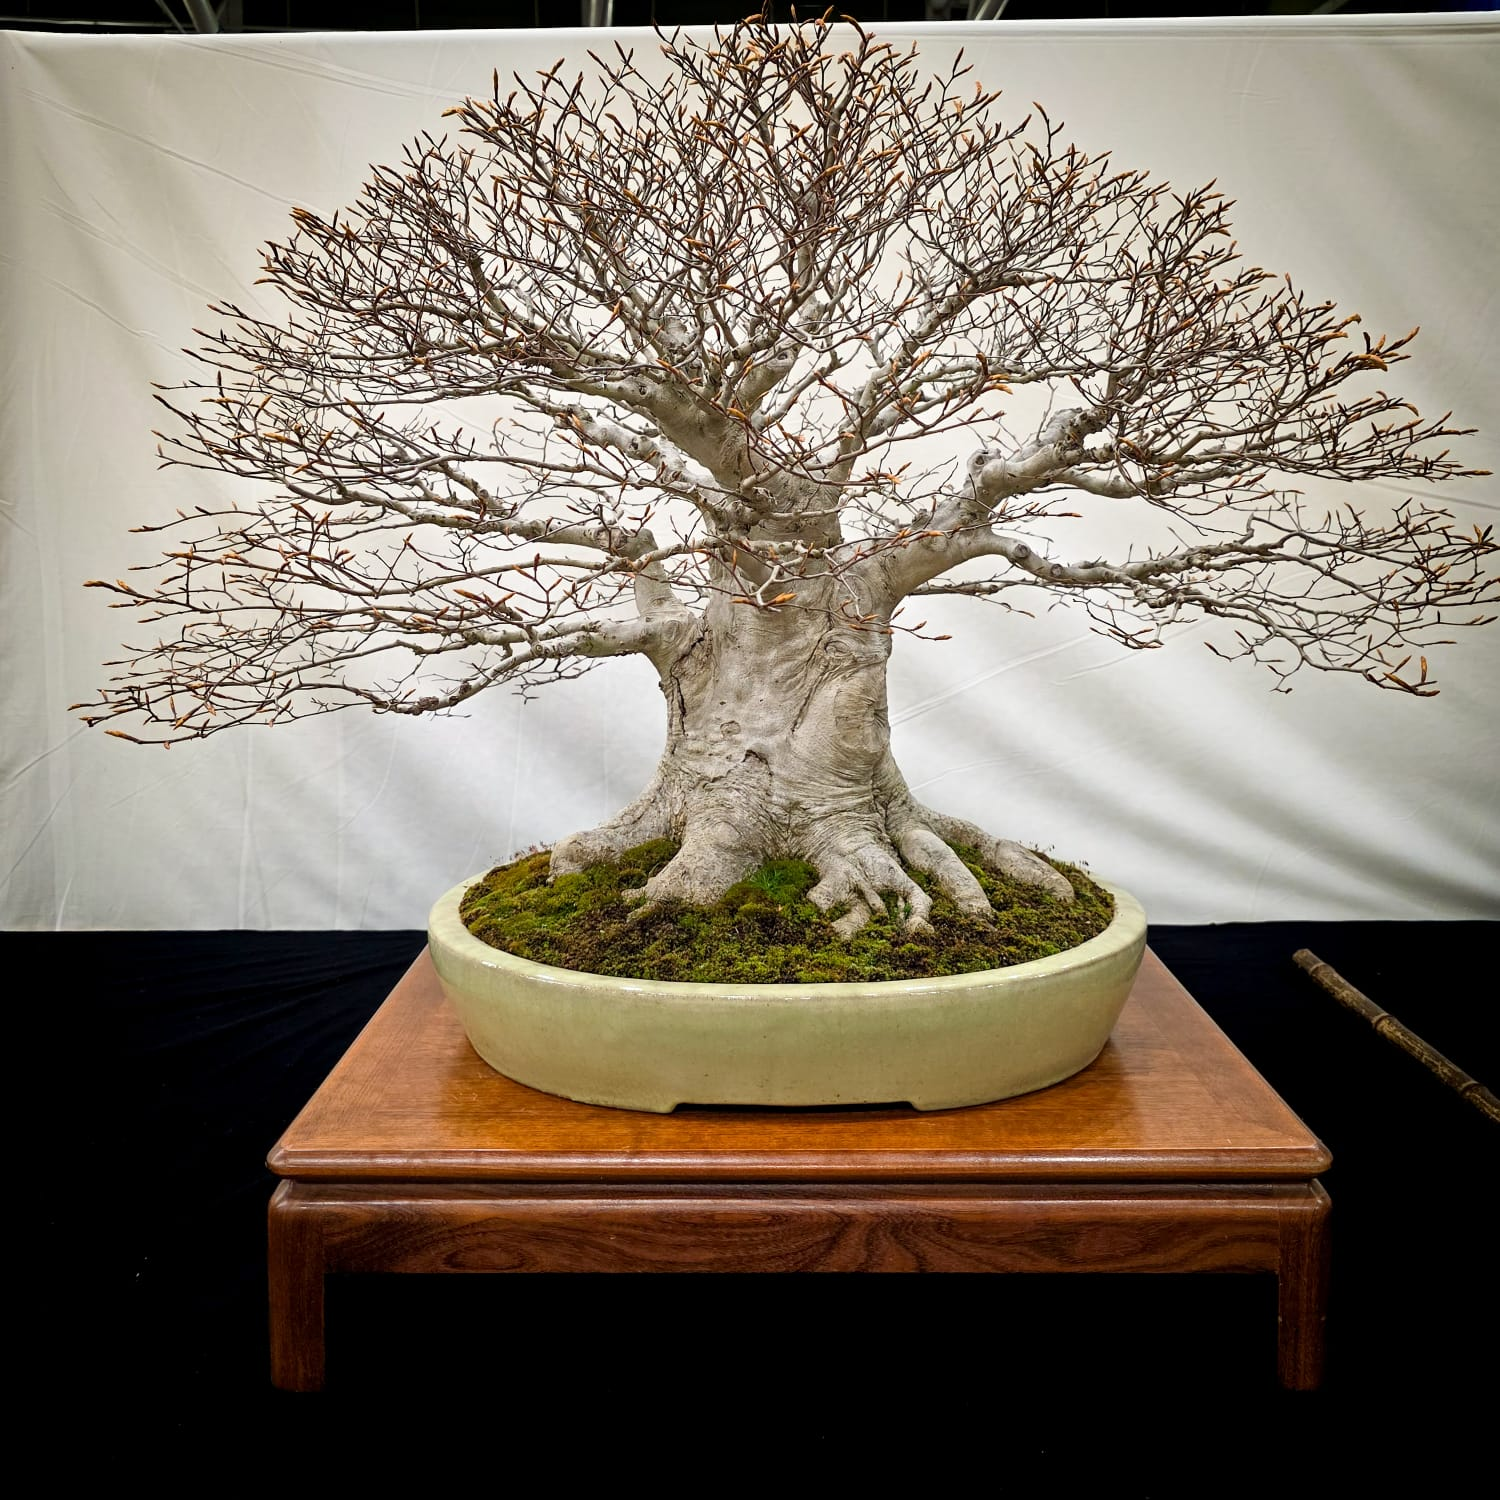
\includegraphics[angle=0,origin=c,width=1.0\textwidth]{2025_05/res/expo_10}
\end{minipage}\quad
\begin{minipage}[b]{.29\textwidth}
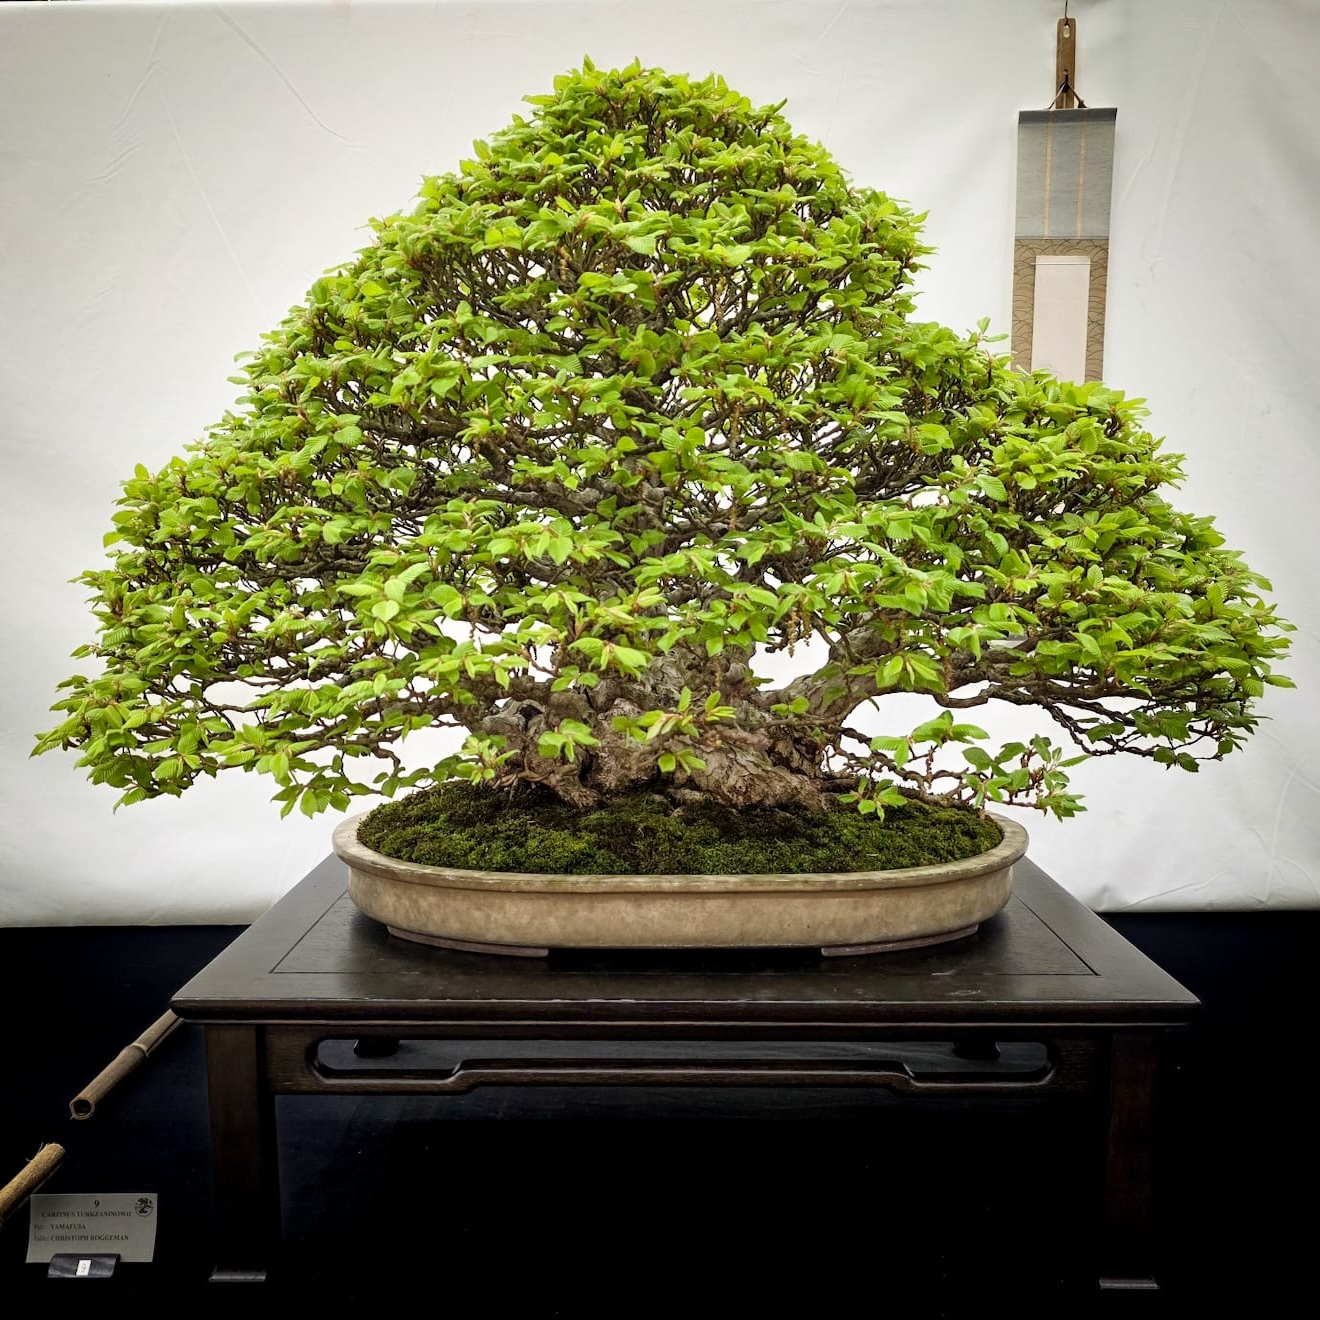
\includegraphics[angle=0,origin=c,width=1.0\textwidth]{2025_05/res/expo_12}
\end{minipage}\quad
\begin{minipage}[b]{.29\textwidth}
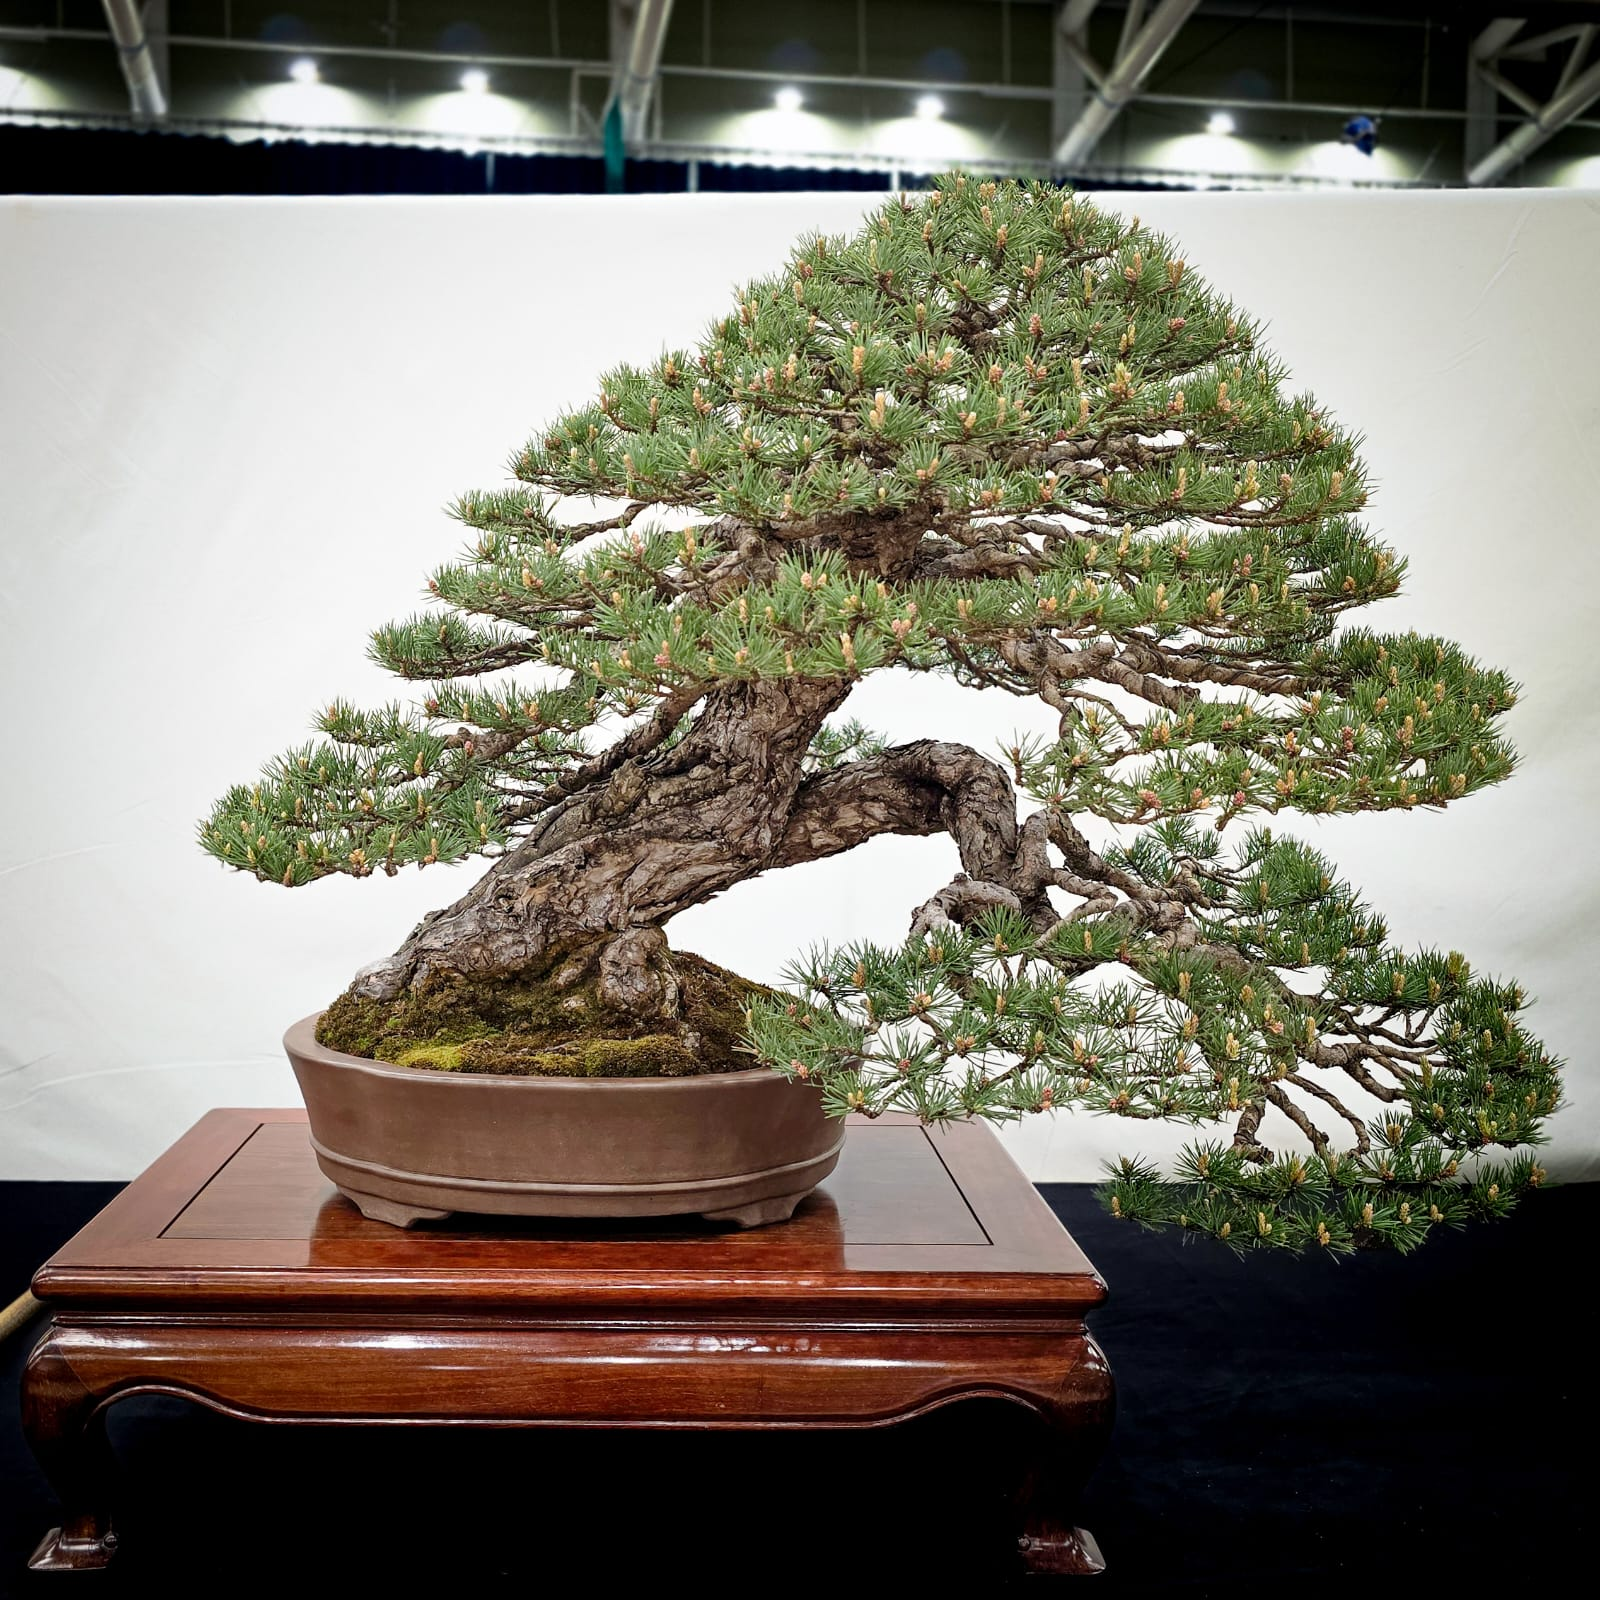
\includegraphics[angle=0,origin=c,width=1.0\textwidth]{2025_05/res/expo_15}
\end{minipage}

\medskip
\begin{minipage}[b]{.29\textwidth}
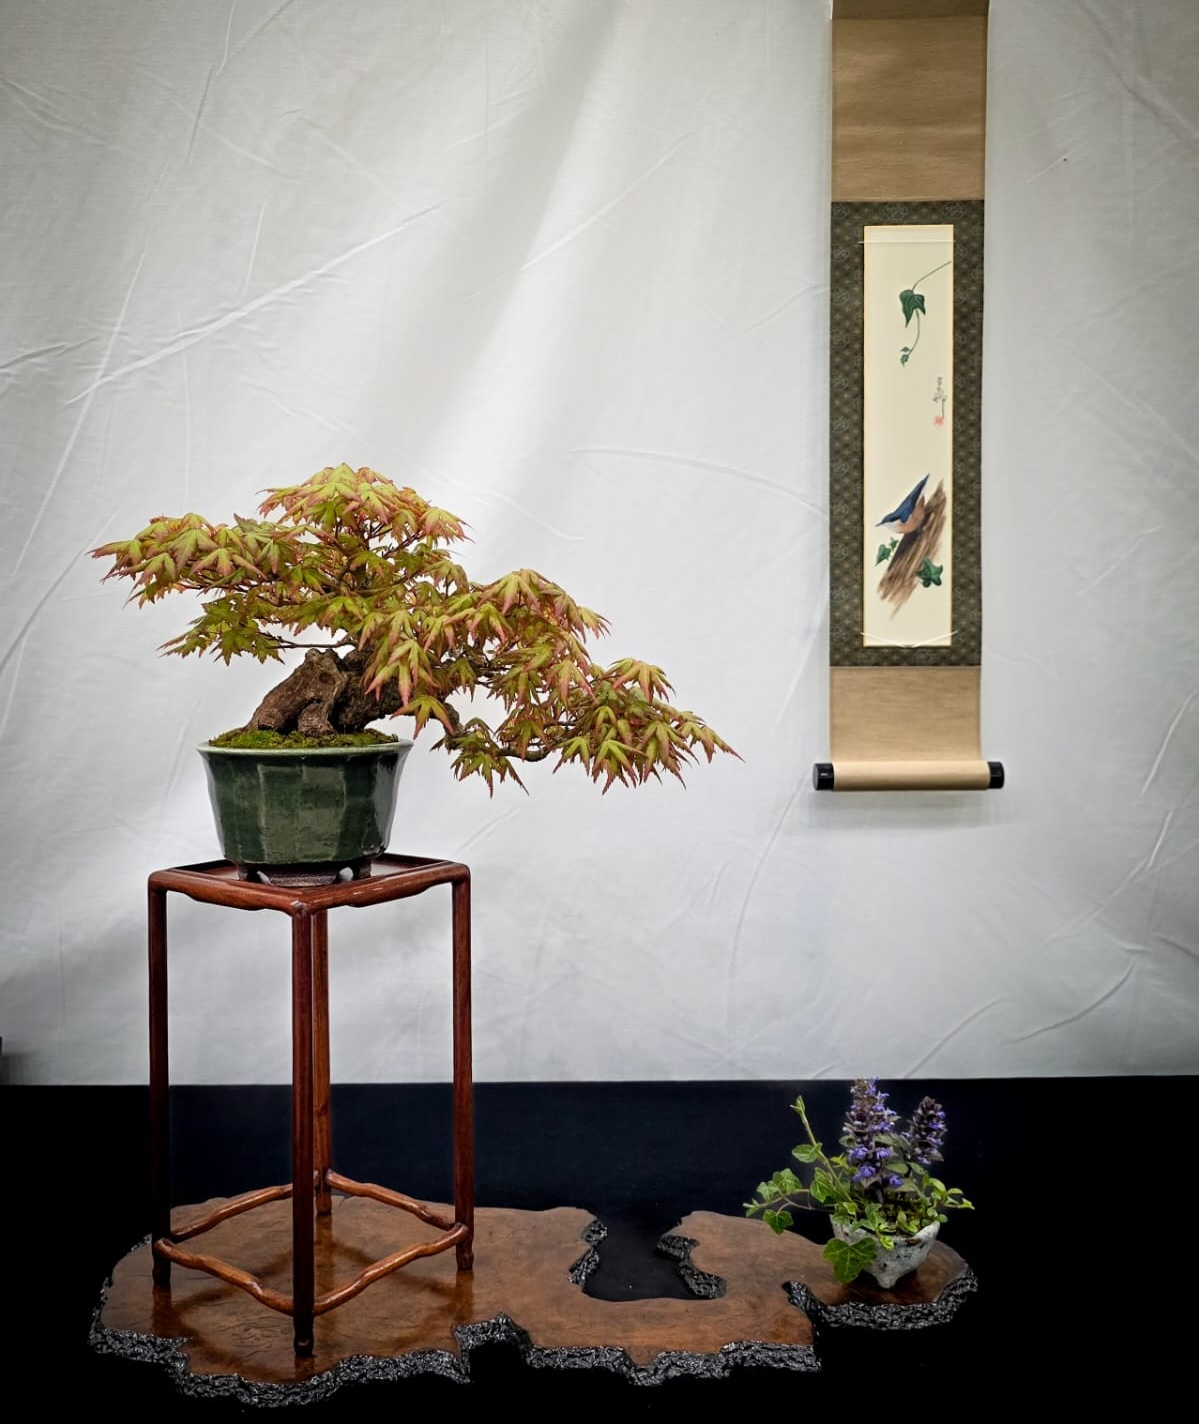
\includegraphics[angle=0,origin=c,width=1.0\textwidth]{2025_05/res/expo_06}
\end{minipage}\quad
\begin{minipage}[b]{.29\textwidth}
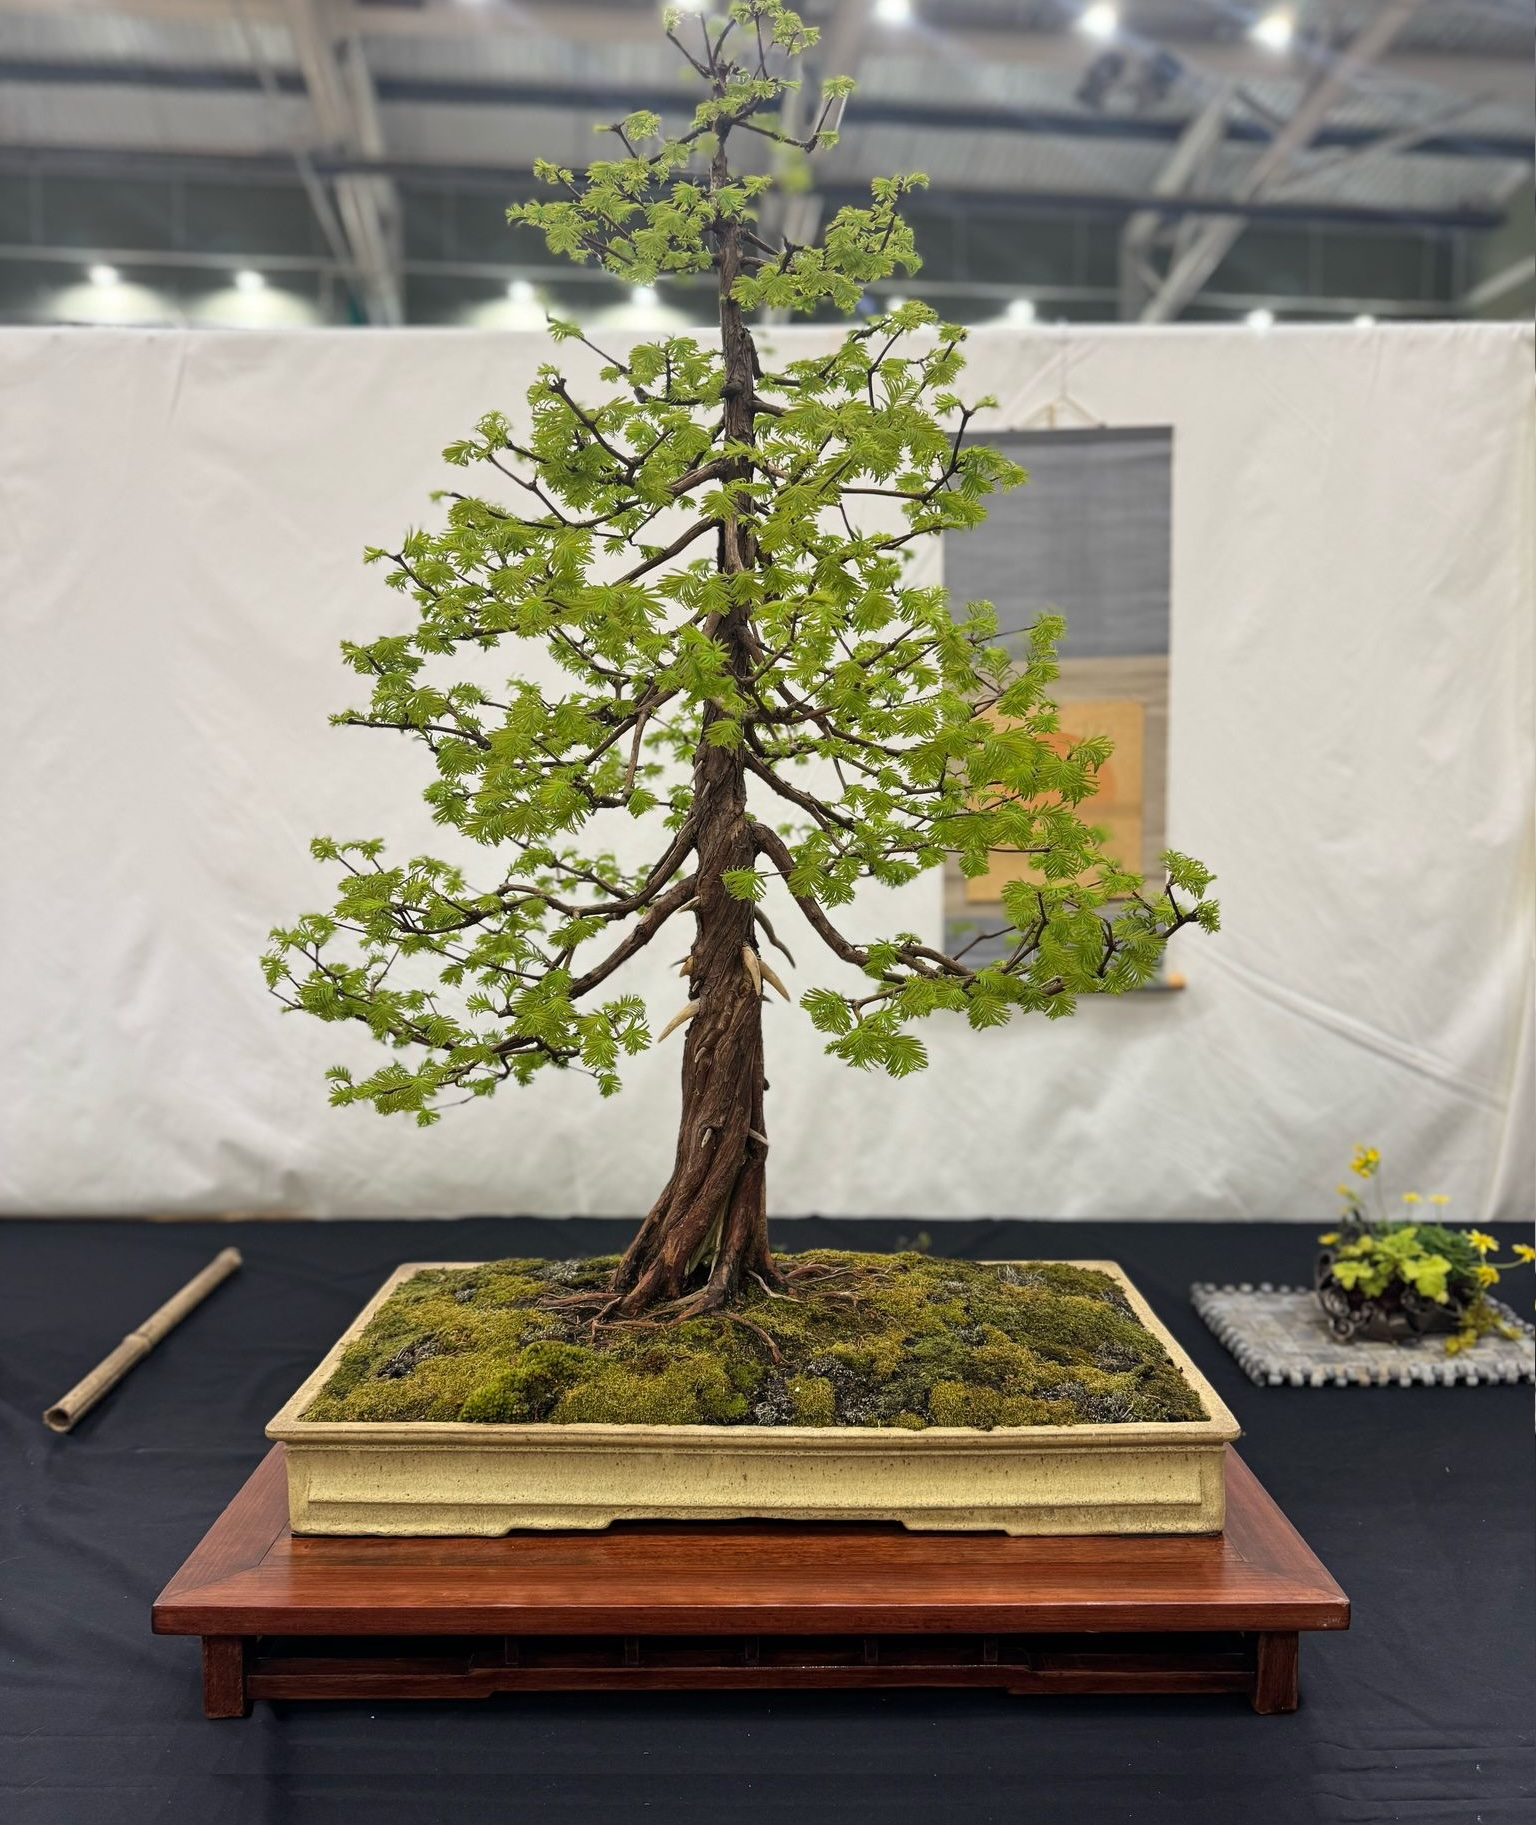
\includegraphics[angle=0,origin=c,width=1.0\textwidth]{2025_05/res/expo_14}
\end{minipage}\quad
\begin{minipage}[b]{.29\textwidth}
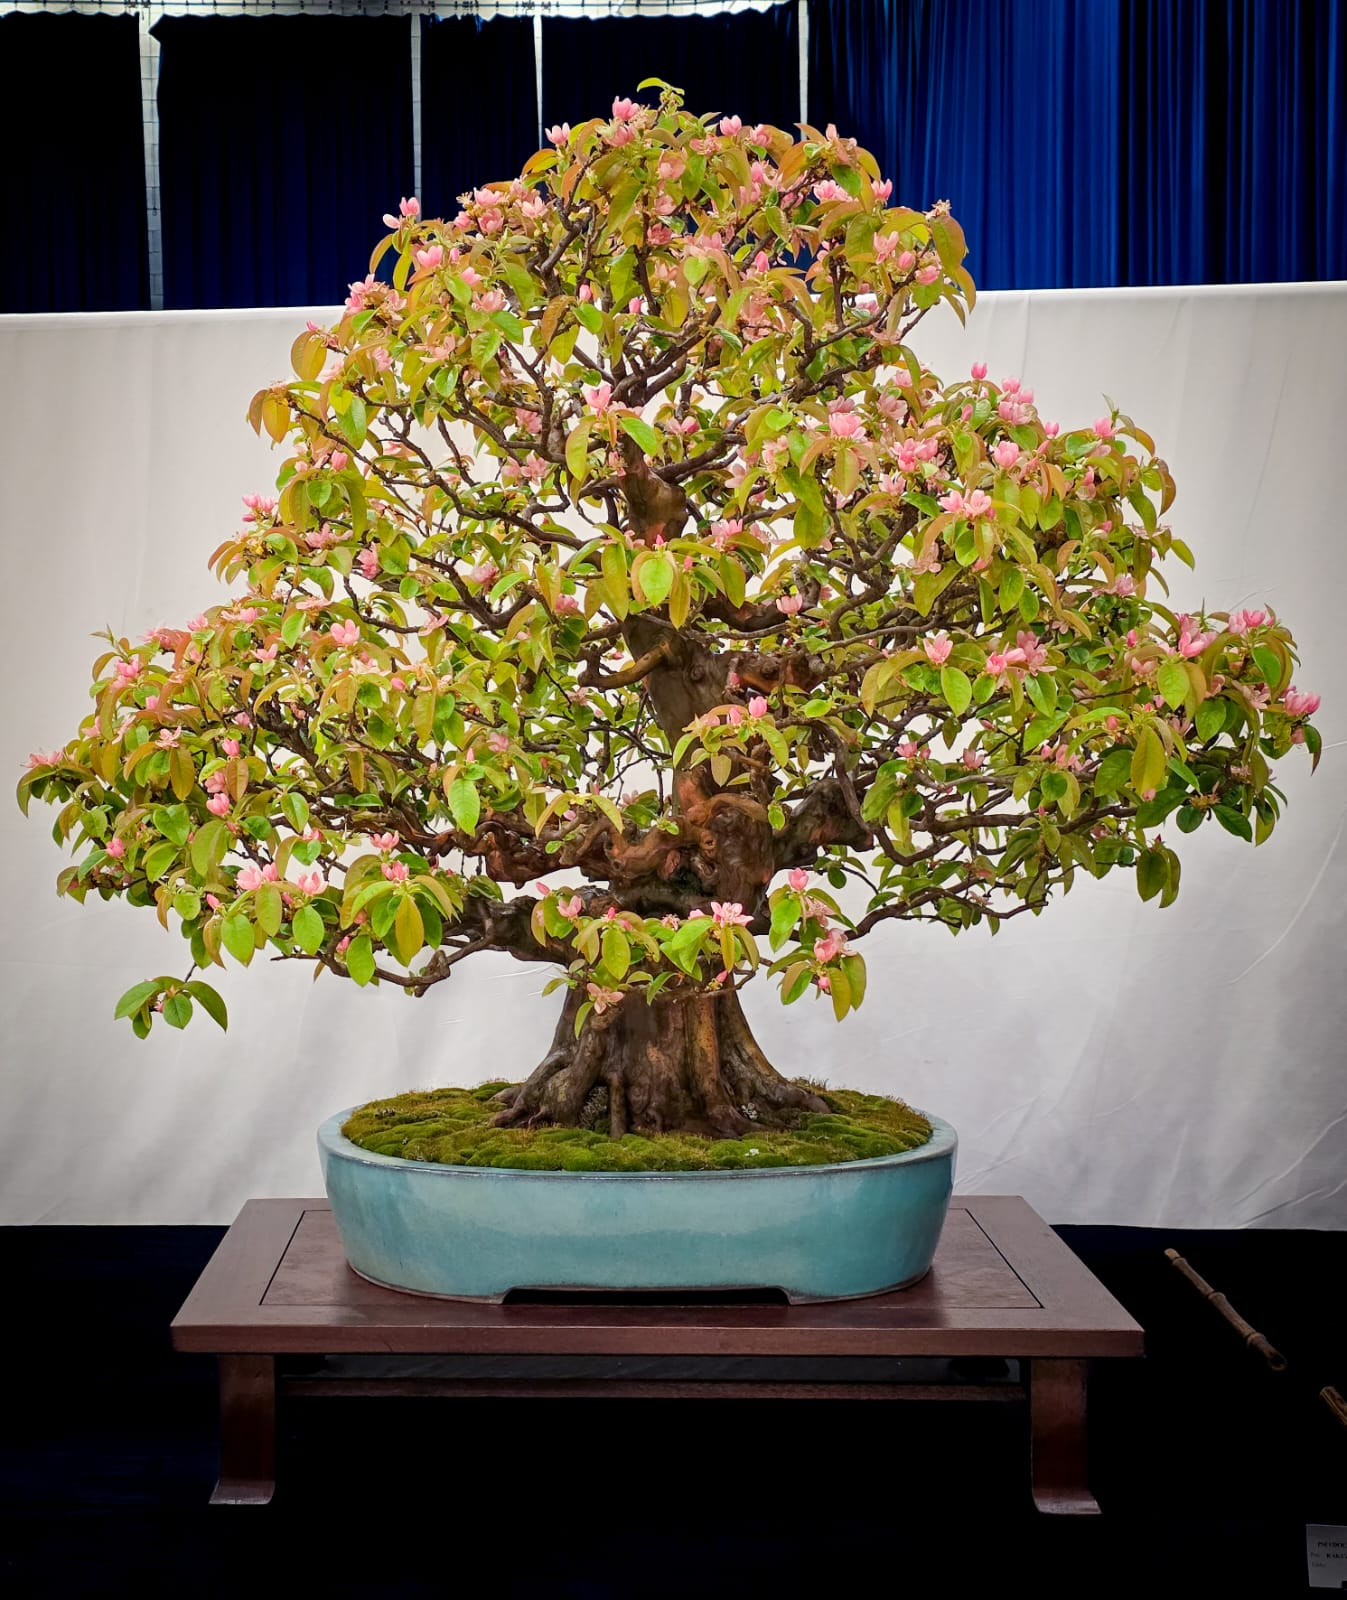
\includegraphics[angle=0,origin=c,width=1.0\textwidth]{2025_05/res/expo_09}
\end{minipage}

\medskip
\begin{minipage}[b]{.29\textwidth}
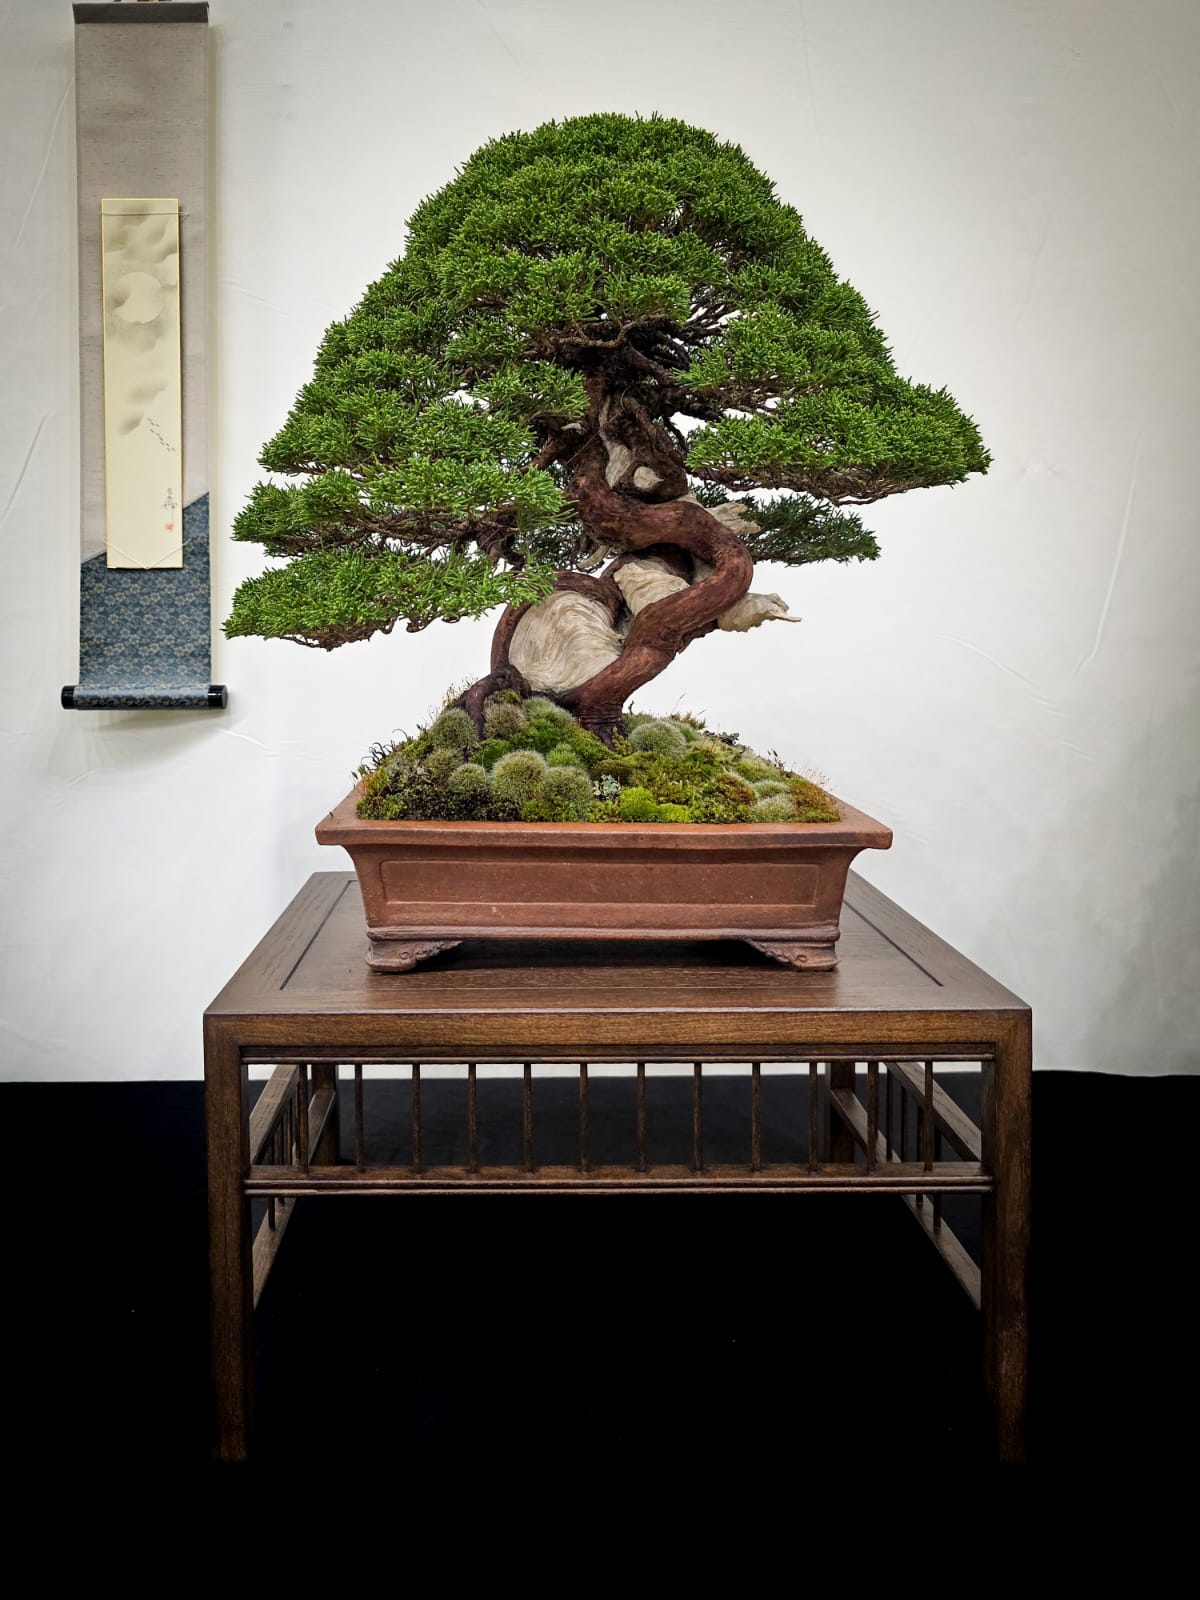
\includegraphics[angle=0,origin=c,width=1.0\textwidth]{2025_05/res/expo_04}
\end{minipage}\quad
\begin{minipage}[b]{.29\textwidth}
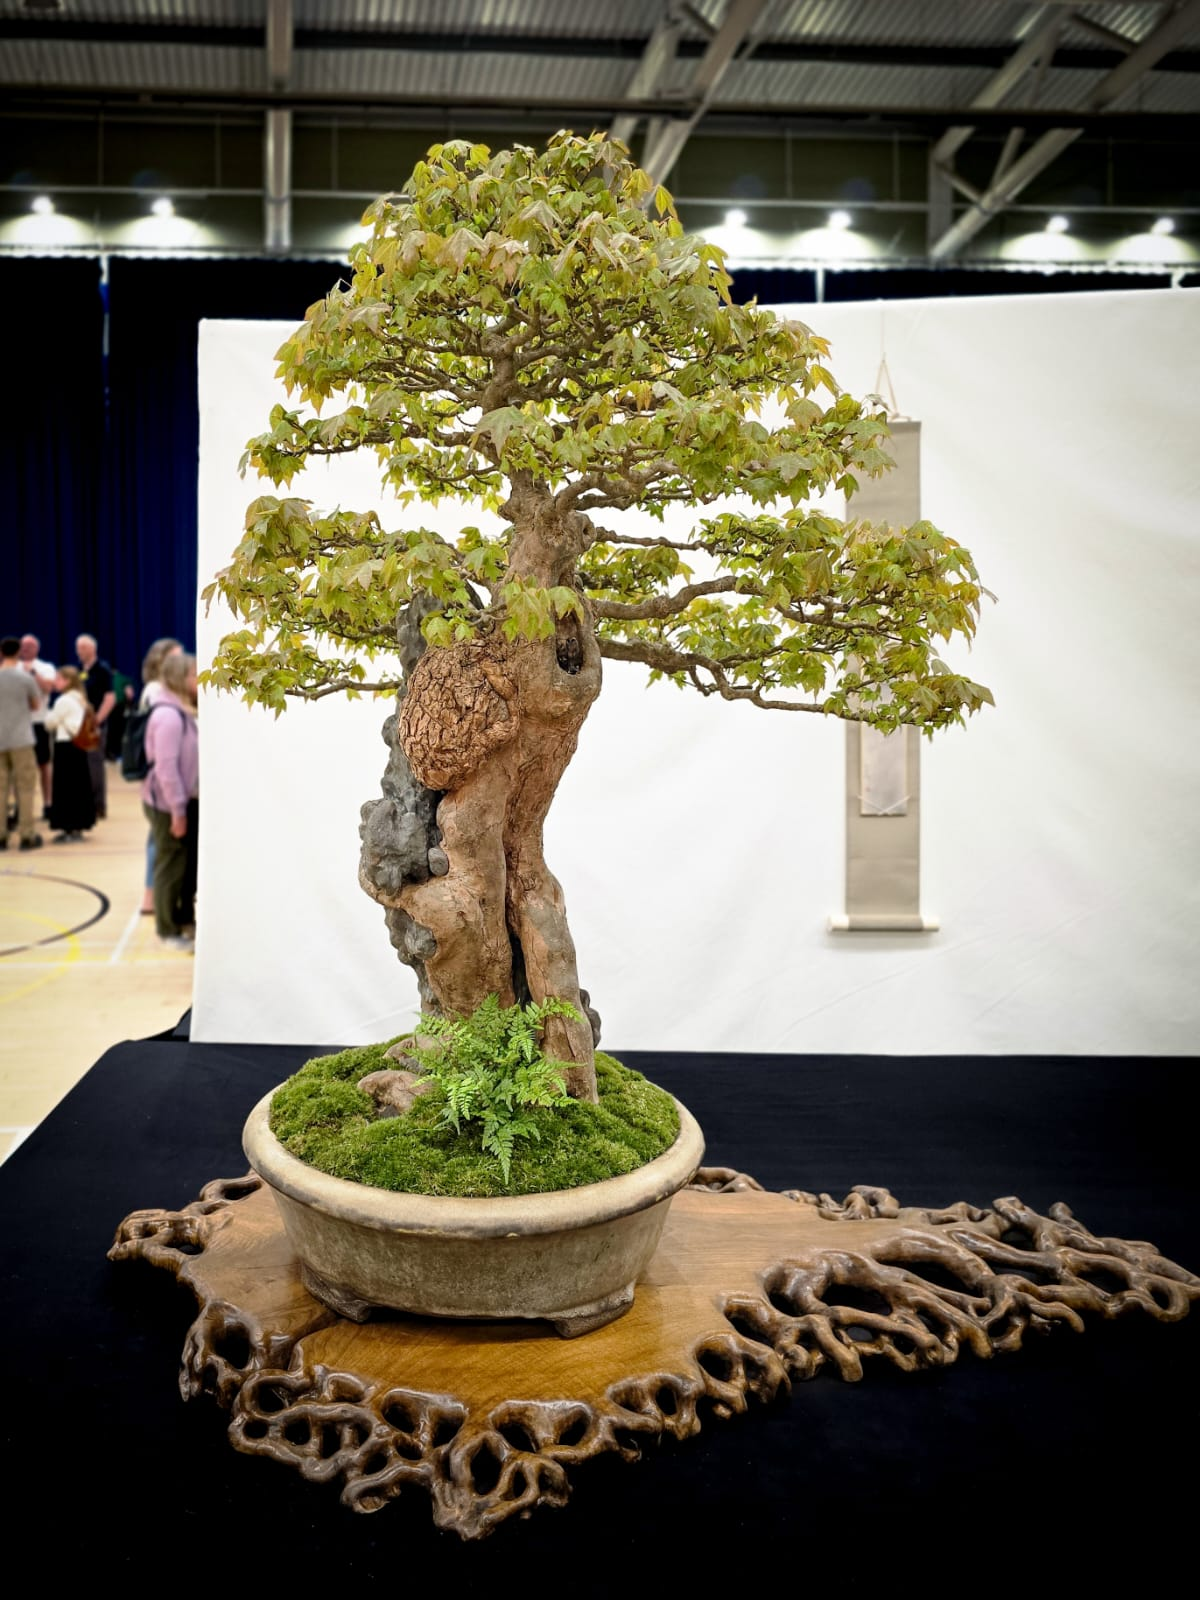
\includegraphics[angle=0,origin=c,width=1.0\textwidth]{2025_05/res/expo_01}
\end{minipage}\quad
\begin{minipage}[b]{.29\textwidth}
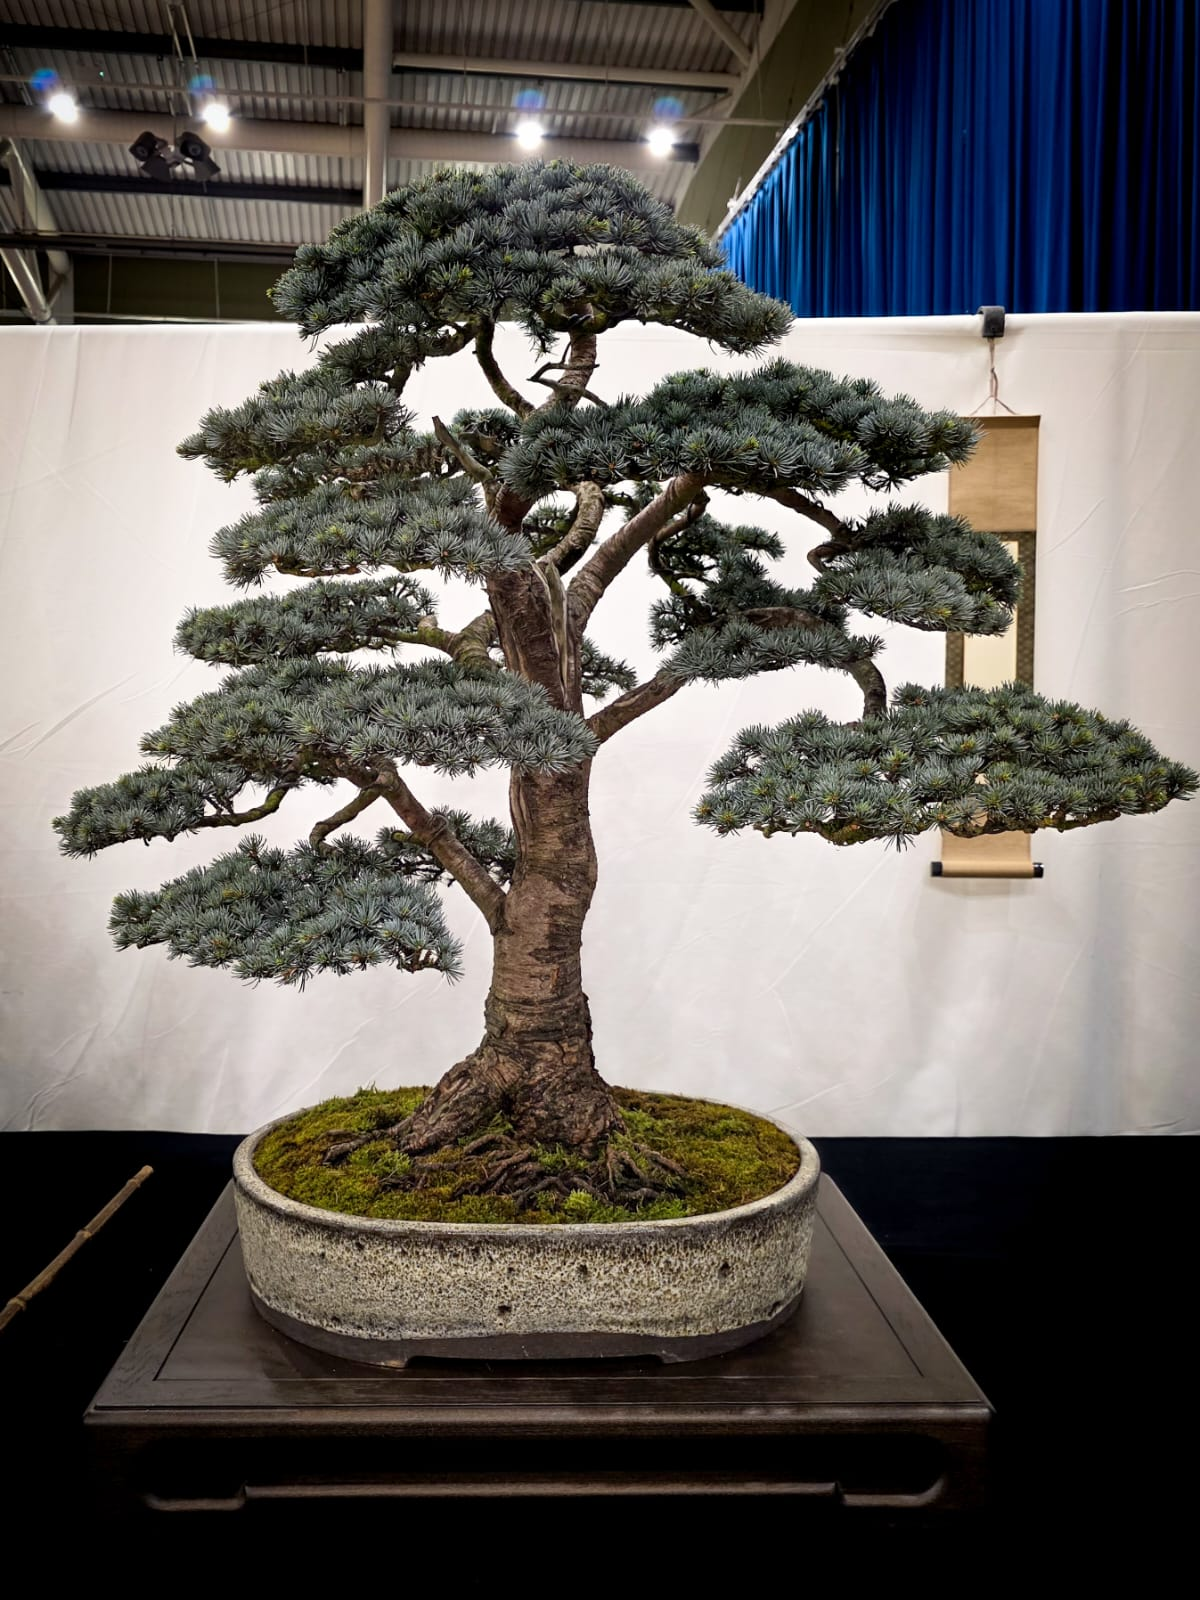
\includegraphics[angle=0,origin=c,width=1.0\textwidth]{2025_05/res/expo_08}
\end{minipage}

\medskip
\emph{A few more pictures of trees displayed at the K2 Bonsai Expo (courtesy of Chris Durne).}
\end{center}
\closearticle
\pagebreak
